% -*- program: pdflatex -*-

\documentclass[11pt]{article}
\usepackage{evolution}
\usepackage[section]{placeins}
\usepackage{geometry}
\usepackage{pdflscape}
 \usepackage{soul}

\begin{document}


\section*{Supplemental information}
\bigskip

\clearpage

%
% FIGURES
%


%Fig S1: Gene 2 tree
\begin{suppfigure}
\centering
\caption{
RdRp gene tree with bootstrap values.
}
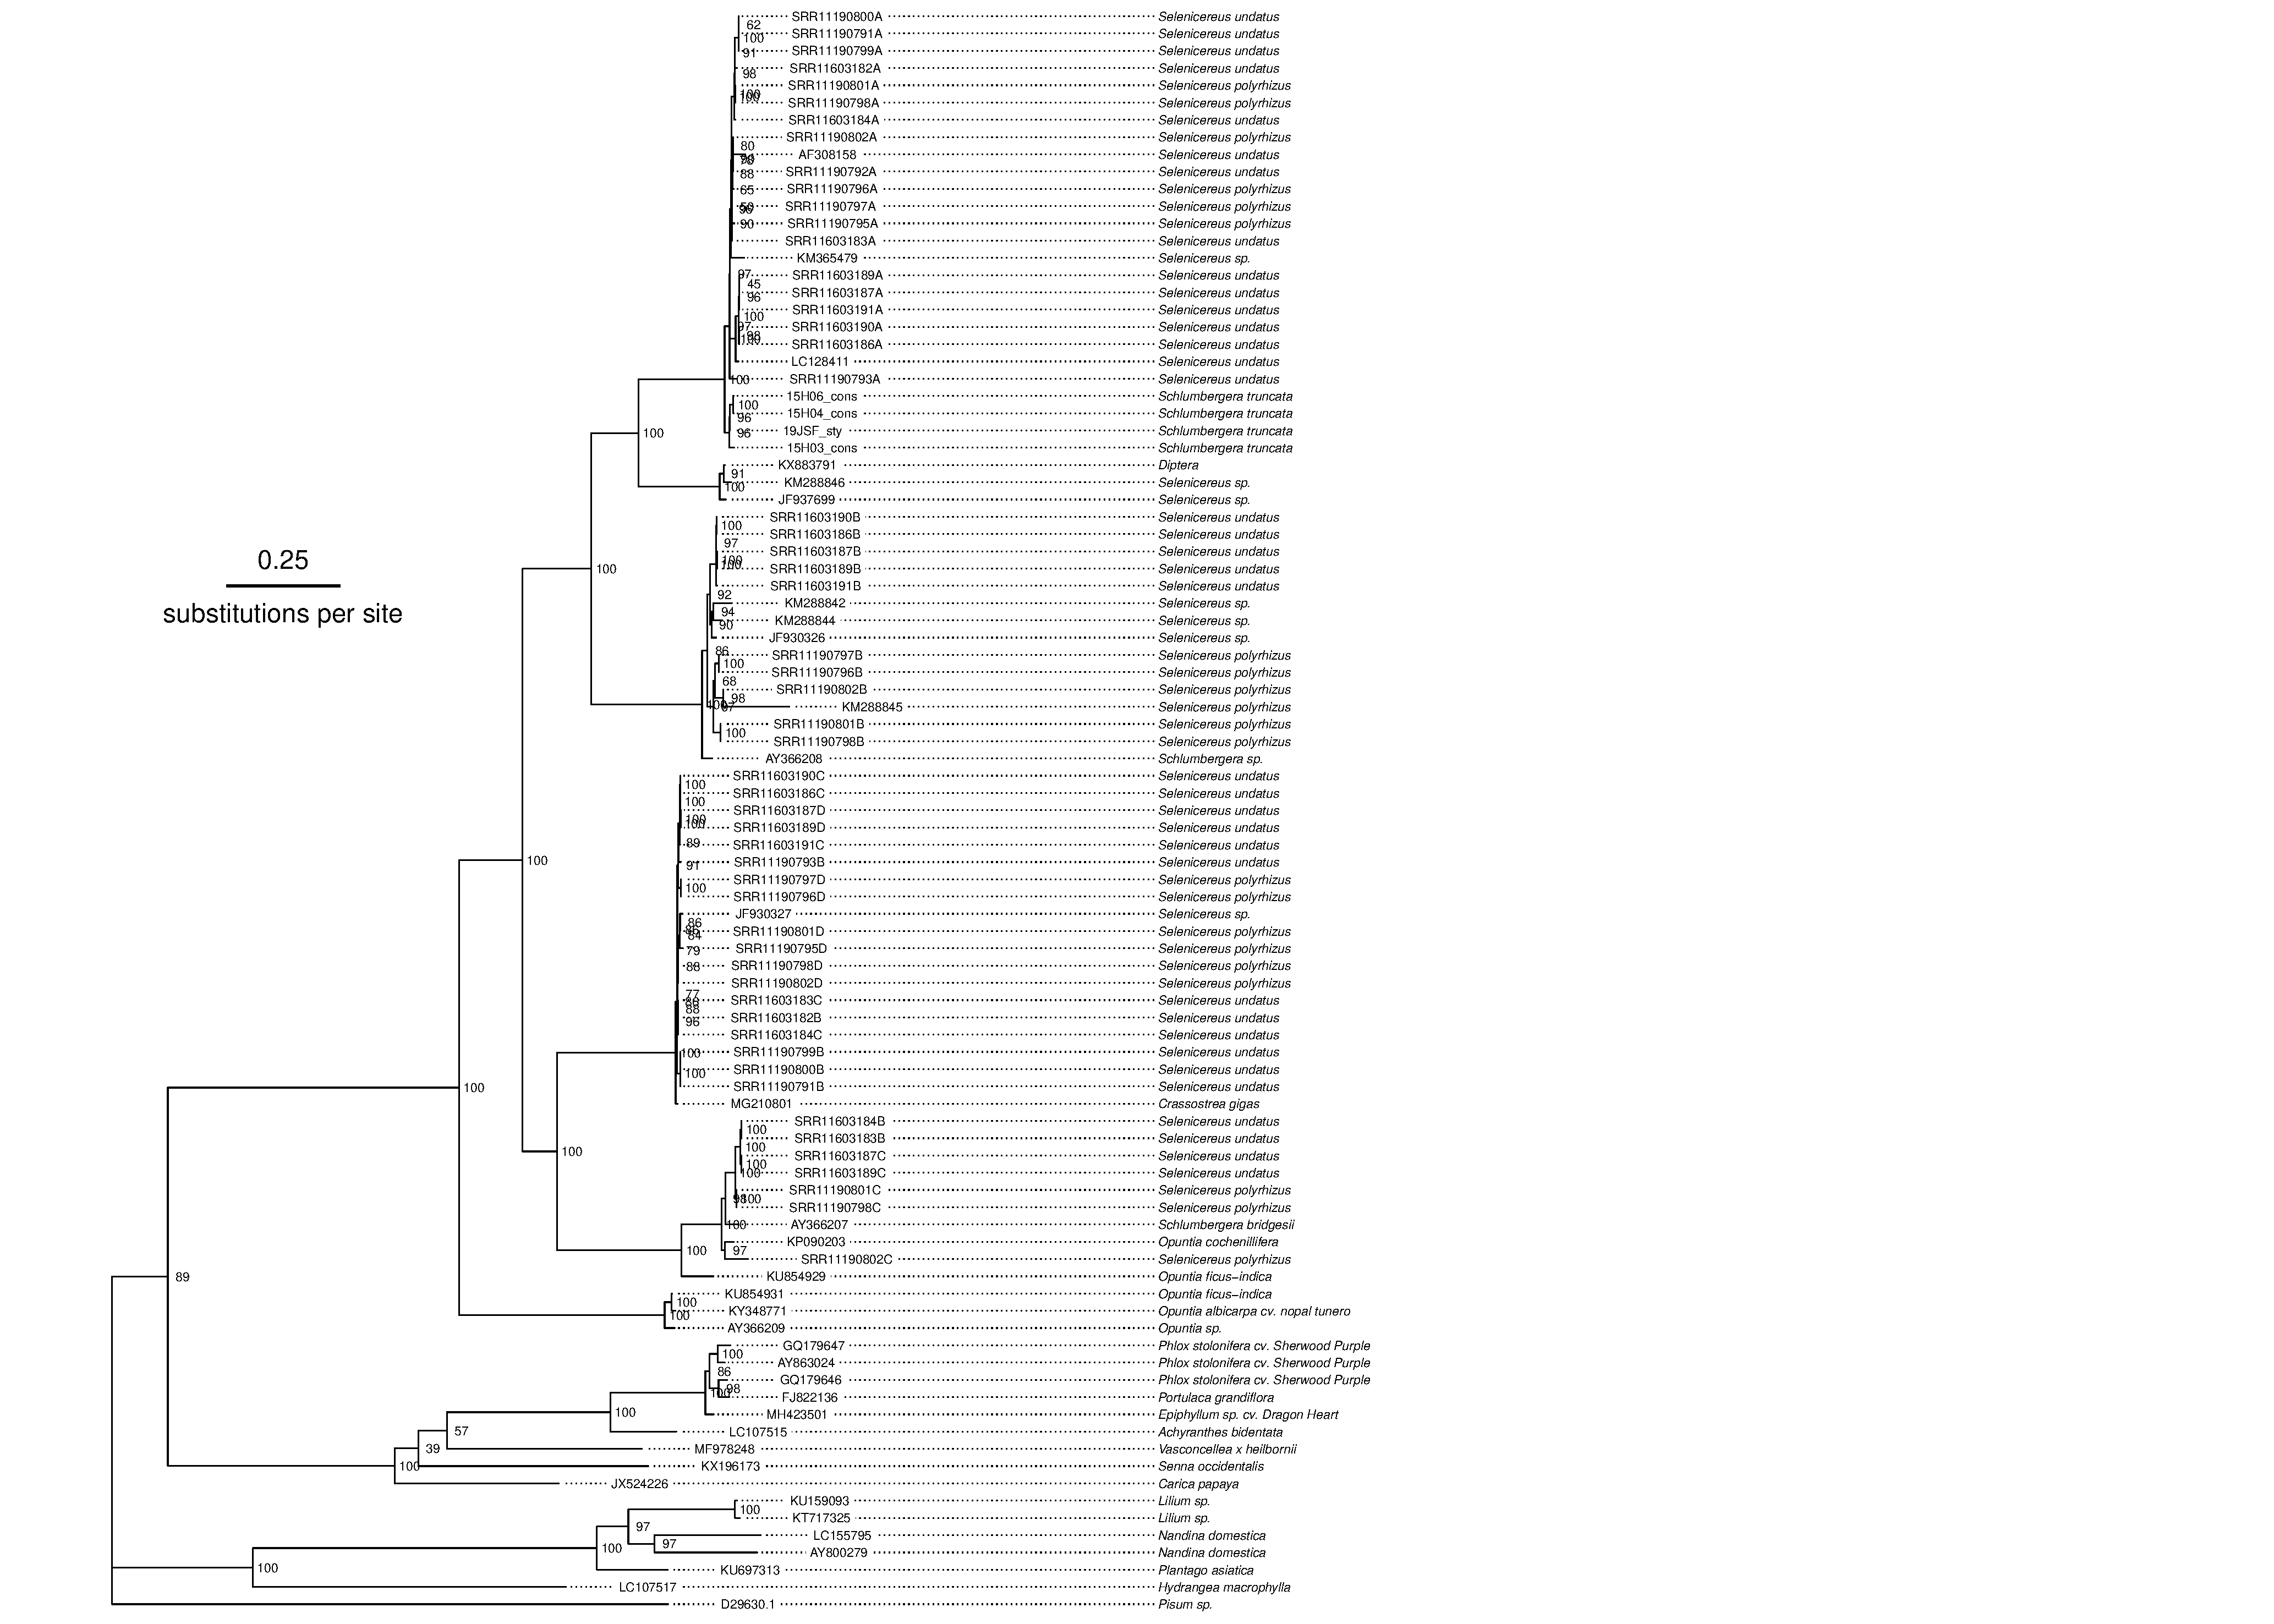
\includegraphics[width=1.5\textwidth]{supplementaryinfo/rdrp_tr.pdf}
\label{fig:genetree2}
\end{suppfigure}
\clearpage


%Fig S2: Gene 2 tree
\begin{suppfigure}
\centering
\caption{
TGB1 gene tree with bootstrap values.
}
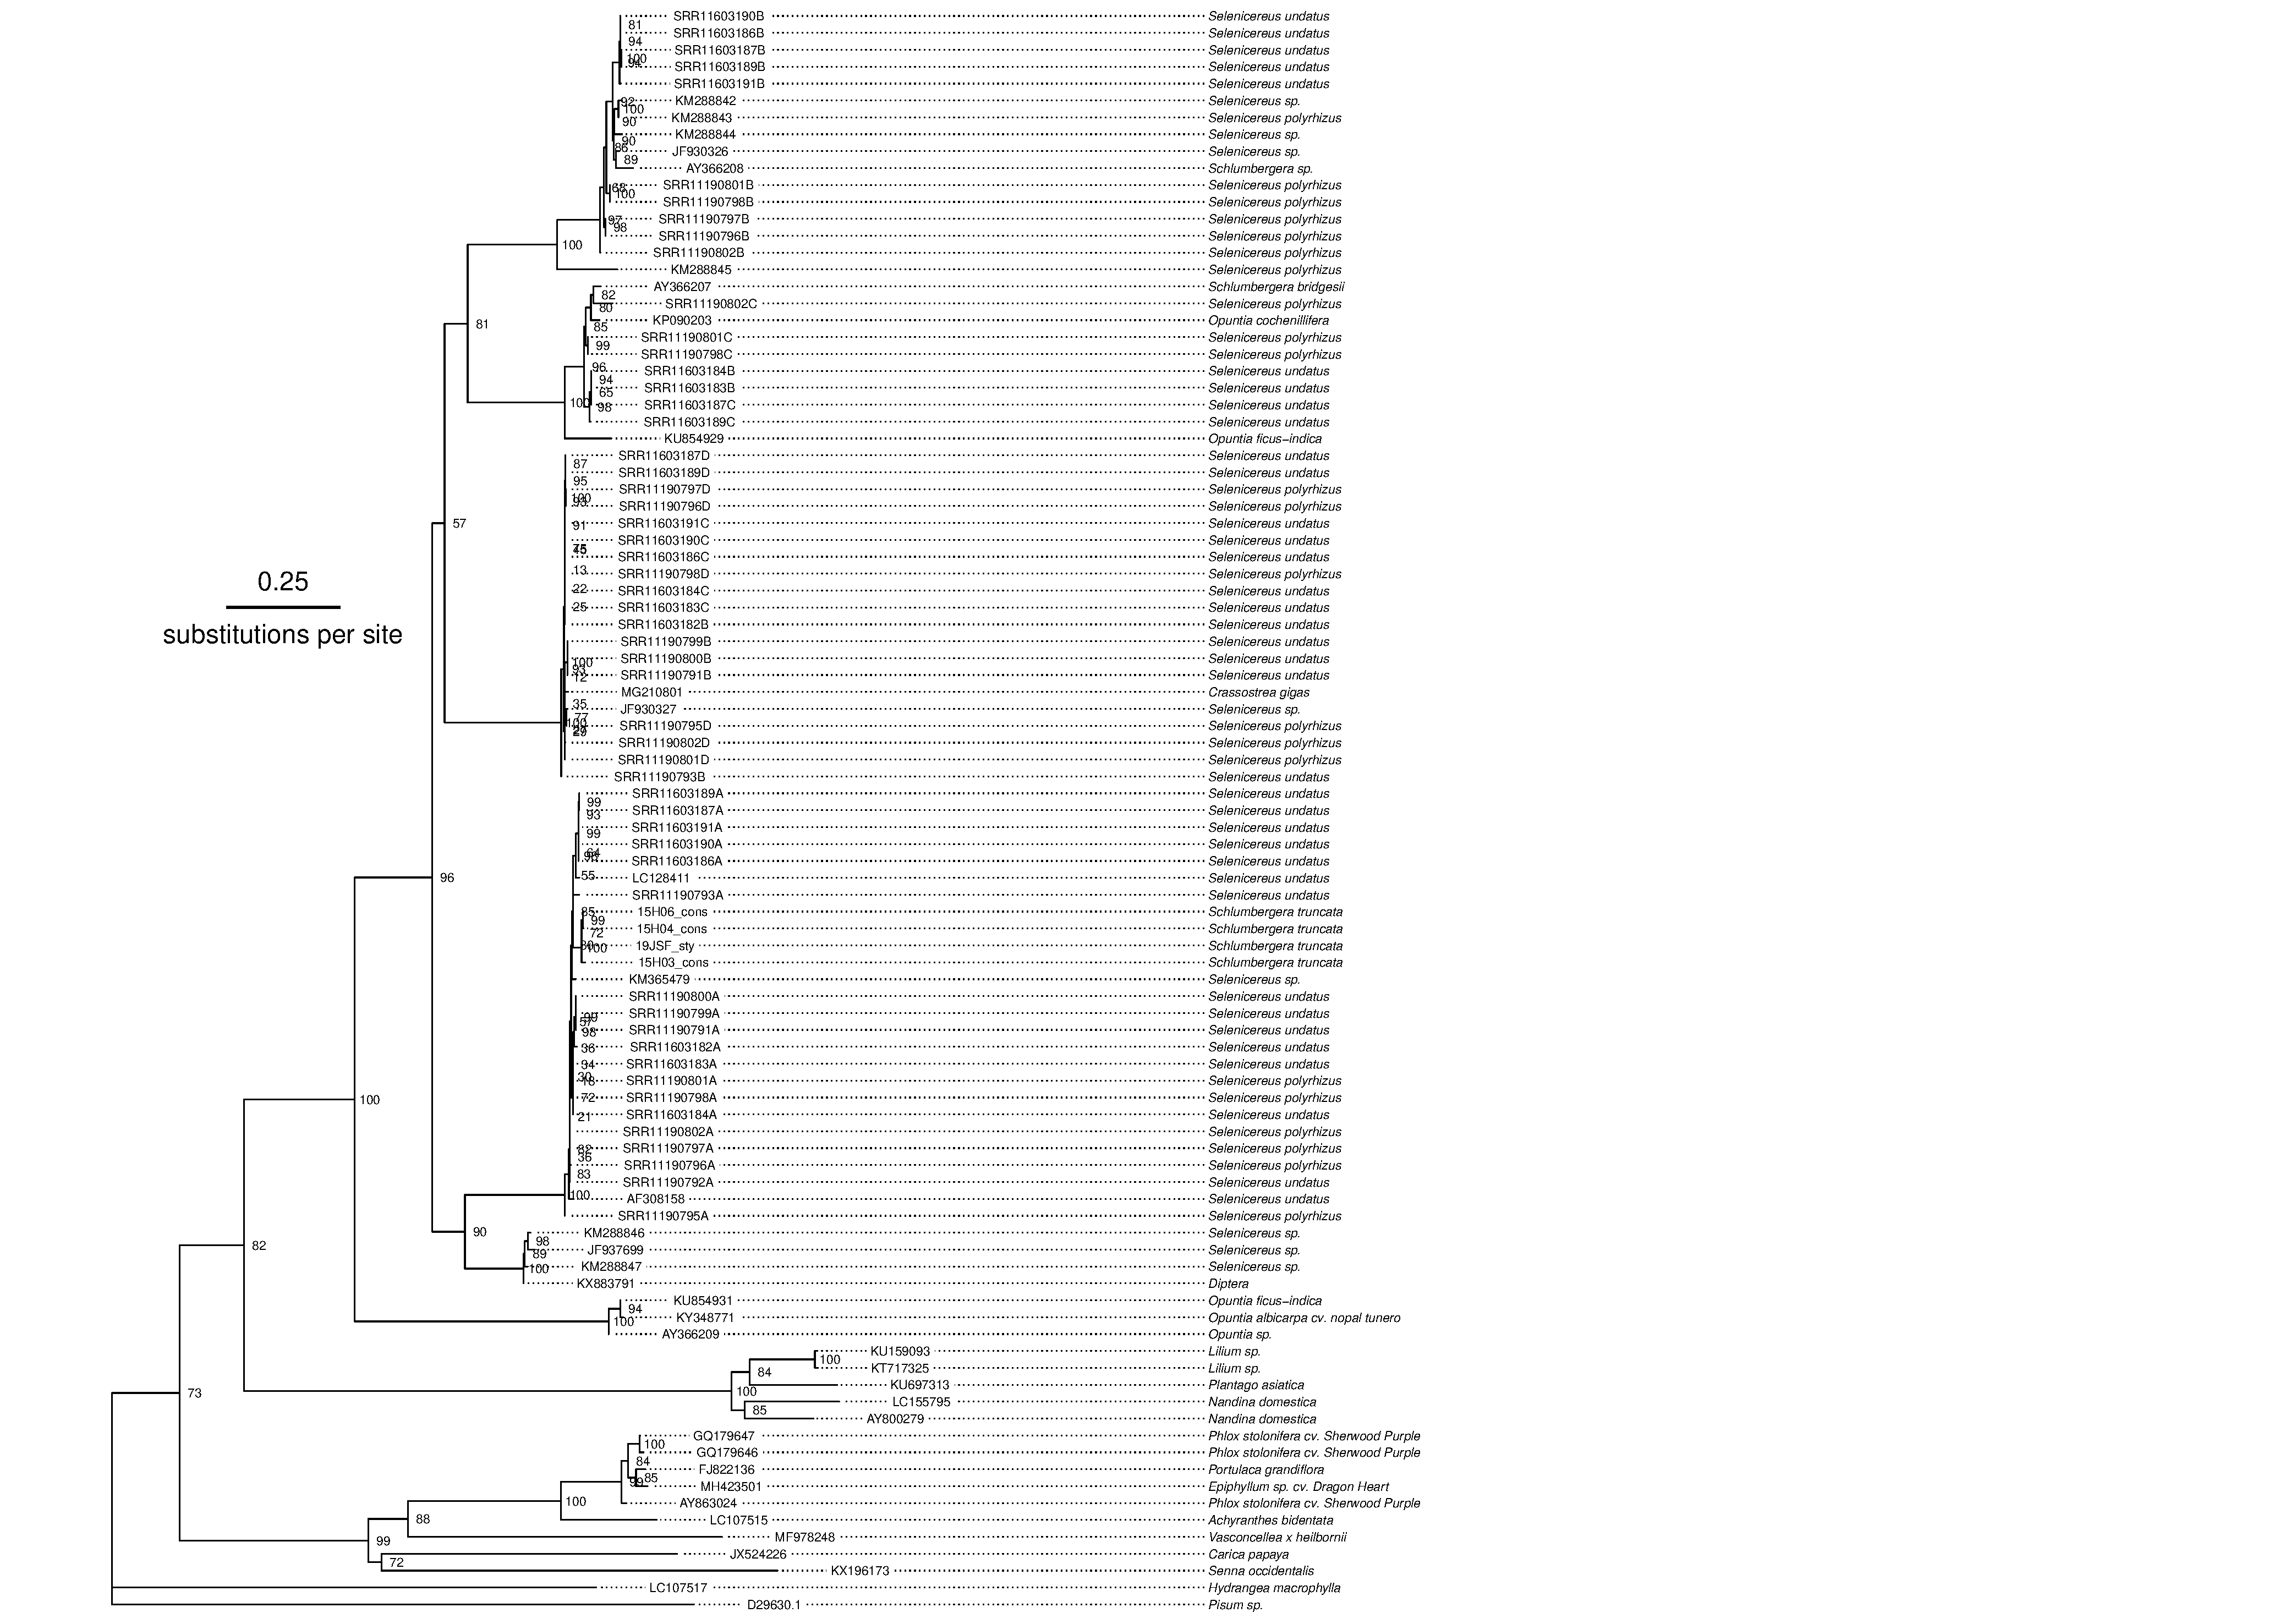
\includegraphics[width=1.5\textwidth]{supplementaryinfo/tgb1_tr.pdf}
\label{fig:genetree2}
\end{suppfigure}
\clearpage

%Fig S3: Gene 3 tree
\begin{suppfigure}
\centering
\caption{
TGB2 gene tree with bootstrap values.
}
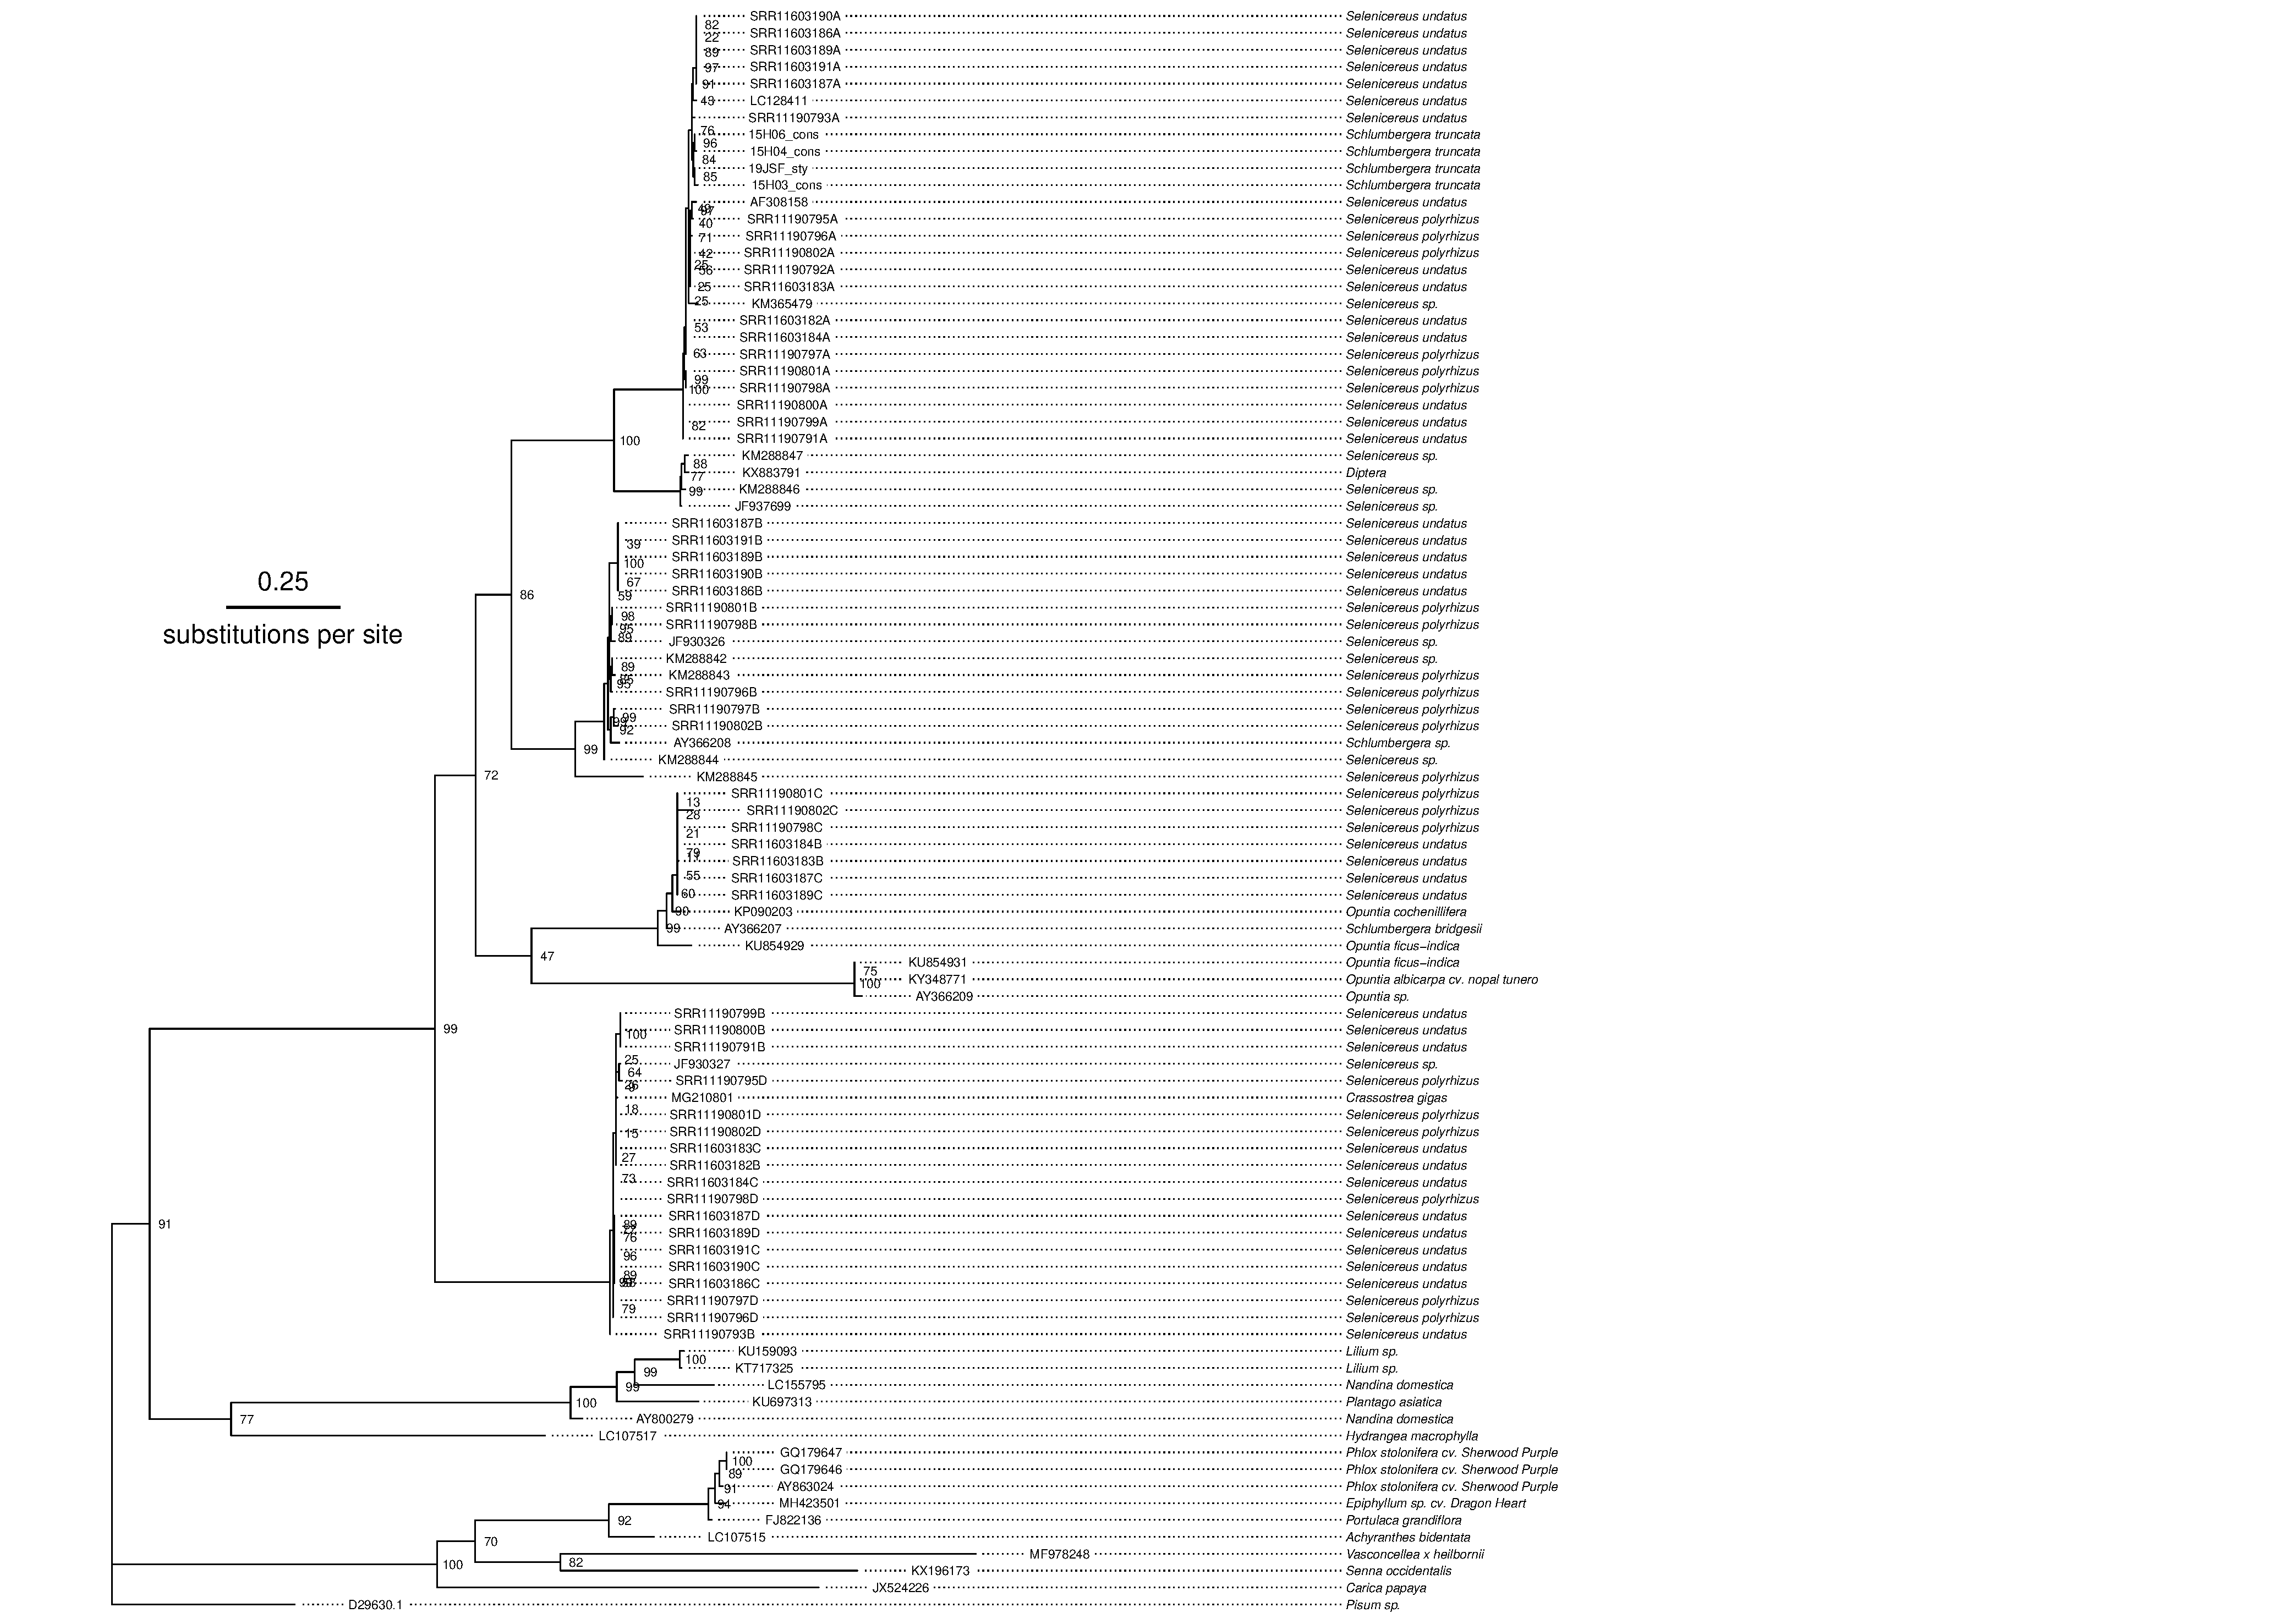
\includegraphics[width=1.5\textwidth]{supplementaryinfo/tgb2_tr.pdf}
\label{fig:genetree3}
\end{suppfigure}
\clearpage

%Fig S4: Gene 4 tree
\begin{suppfigure}
\centering
\caption{
TGB3 gene tree with bootstrap values.
}
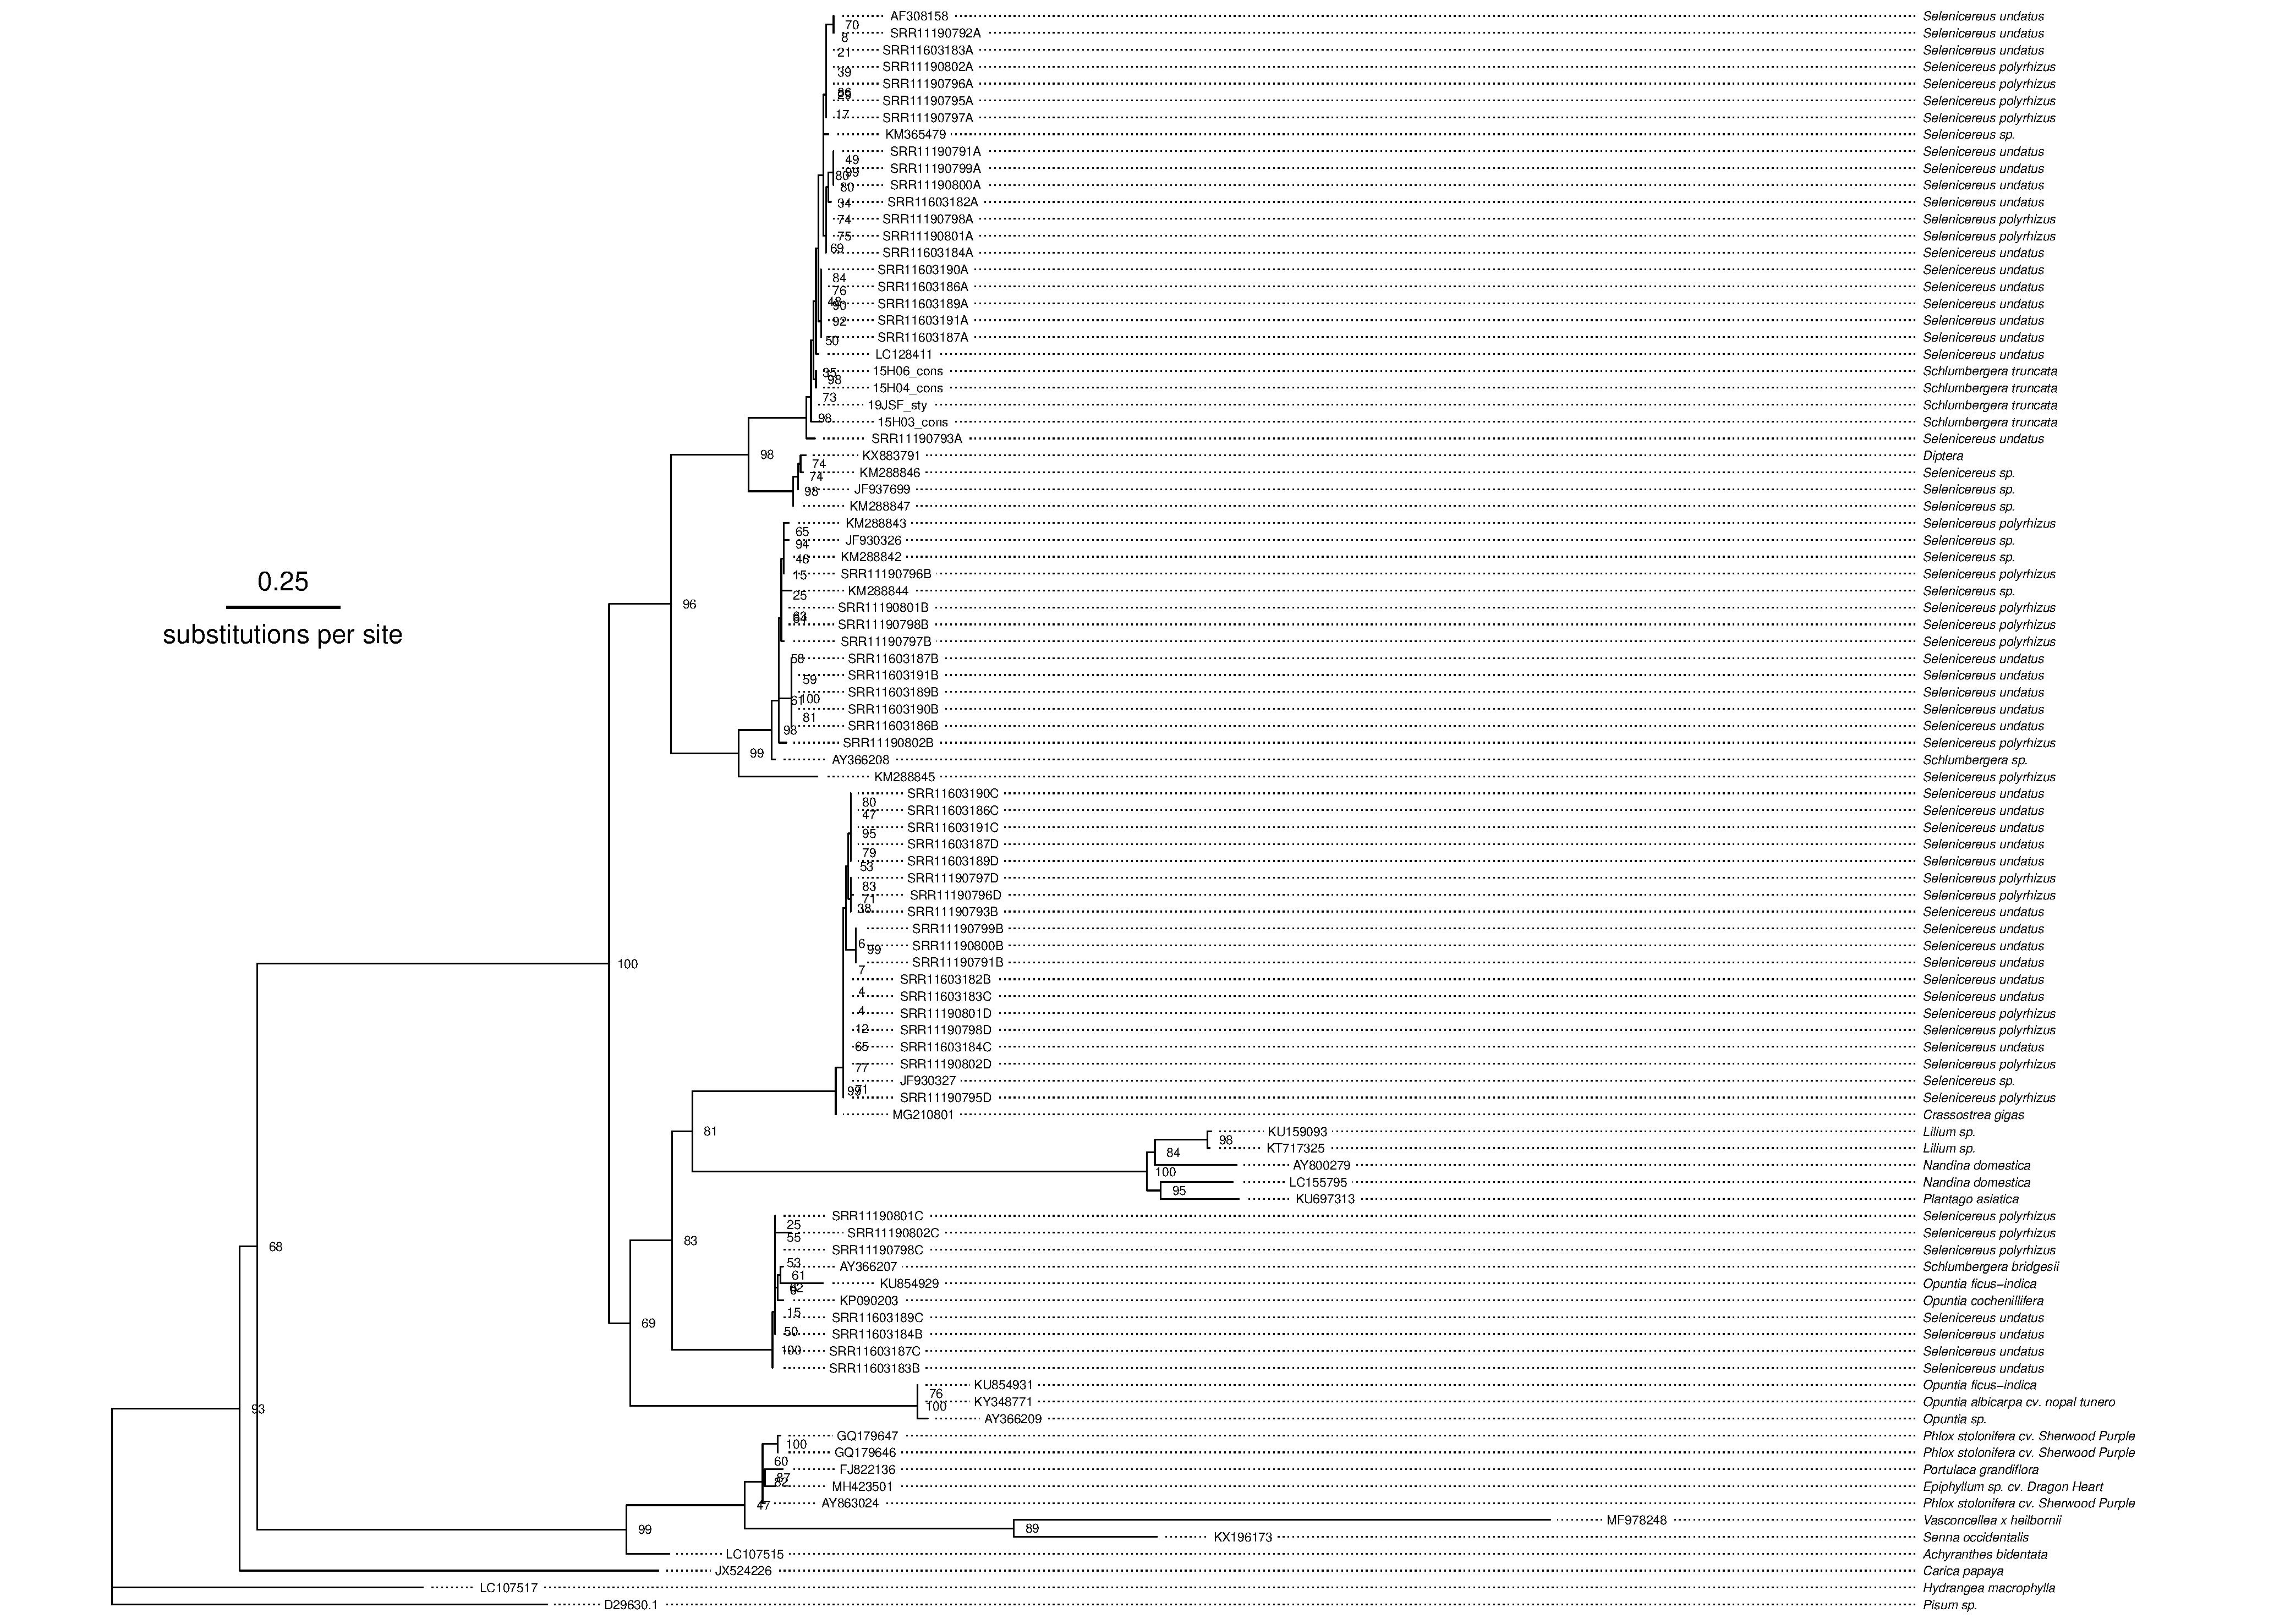
\includegraphics[width=1.2\textwidth]{supplementaryinfo/tgb3_tr.pdf}
\label{fig:genetree4}
\end{suppfigure}
\clearpage

%Fig S5: Gene 5 tree
\begin{suppfigure}
\centering
\caption{
CP gene tree with bootstrap values.
}
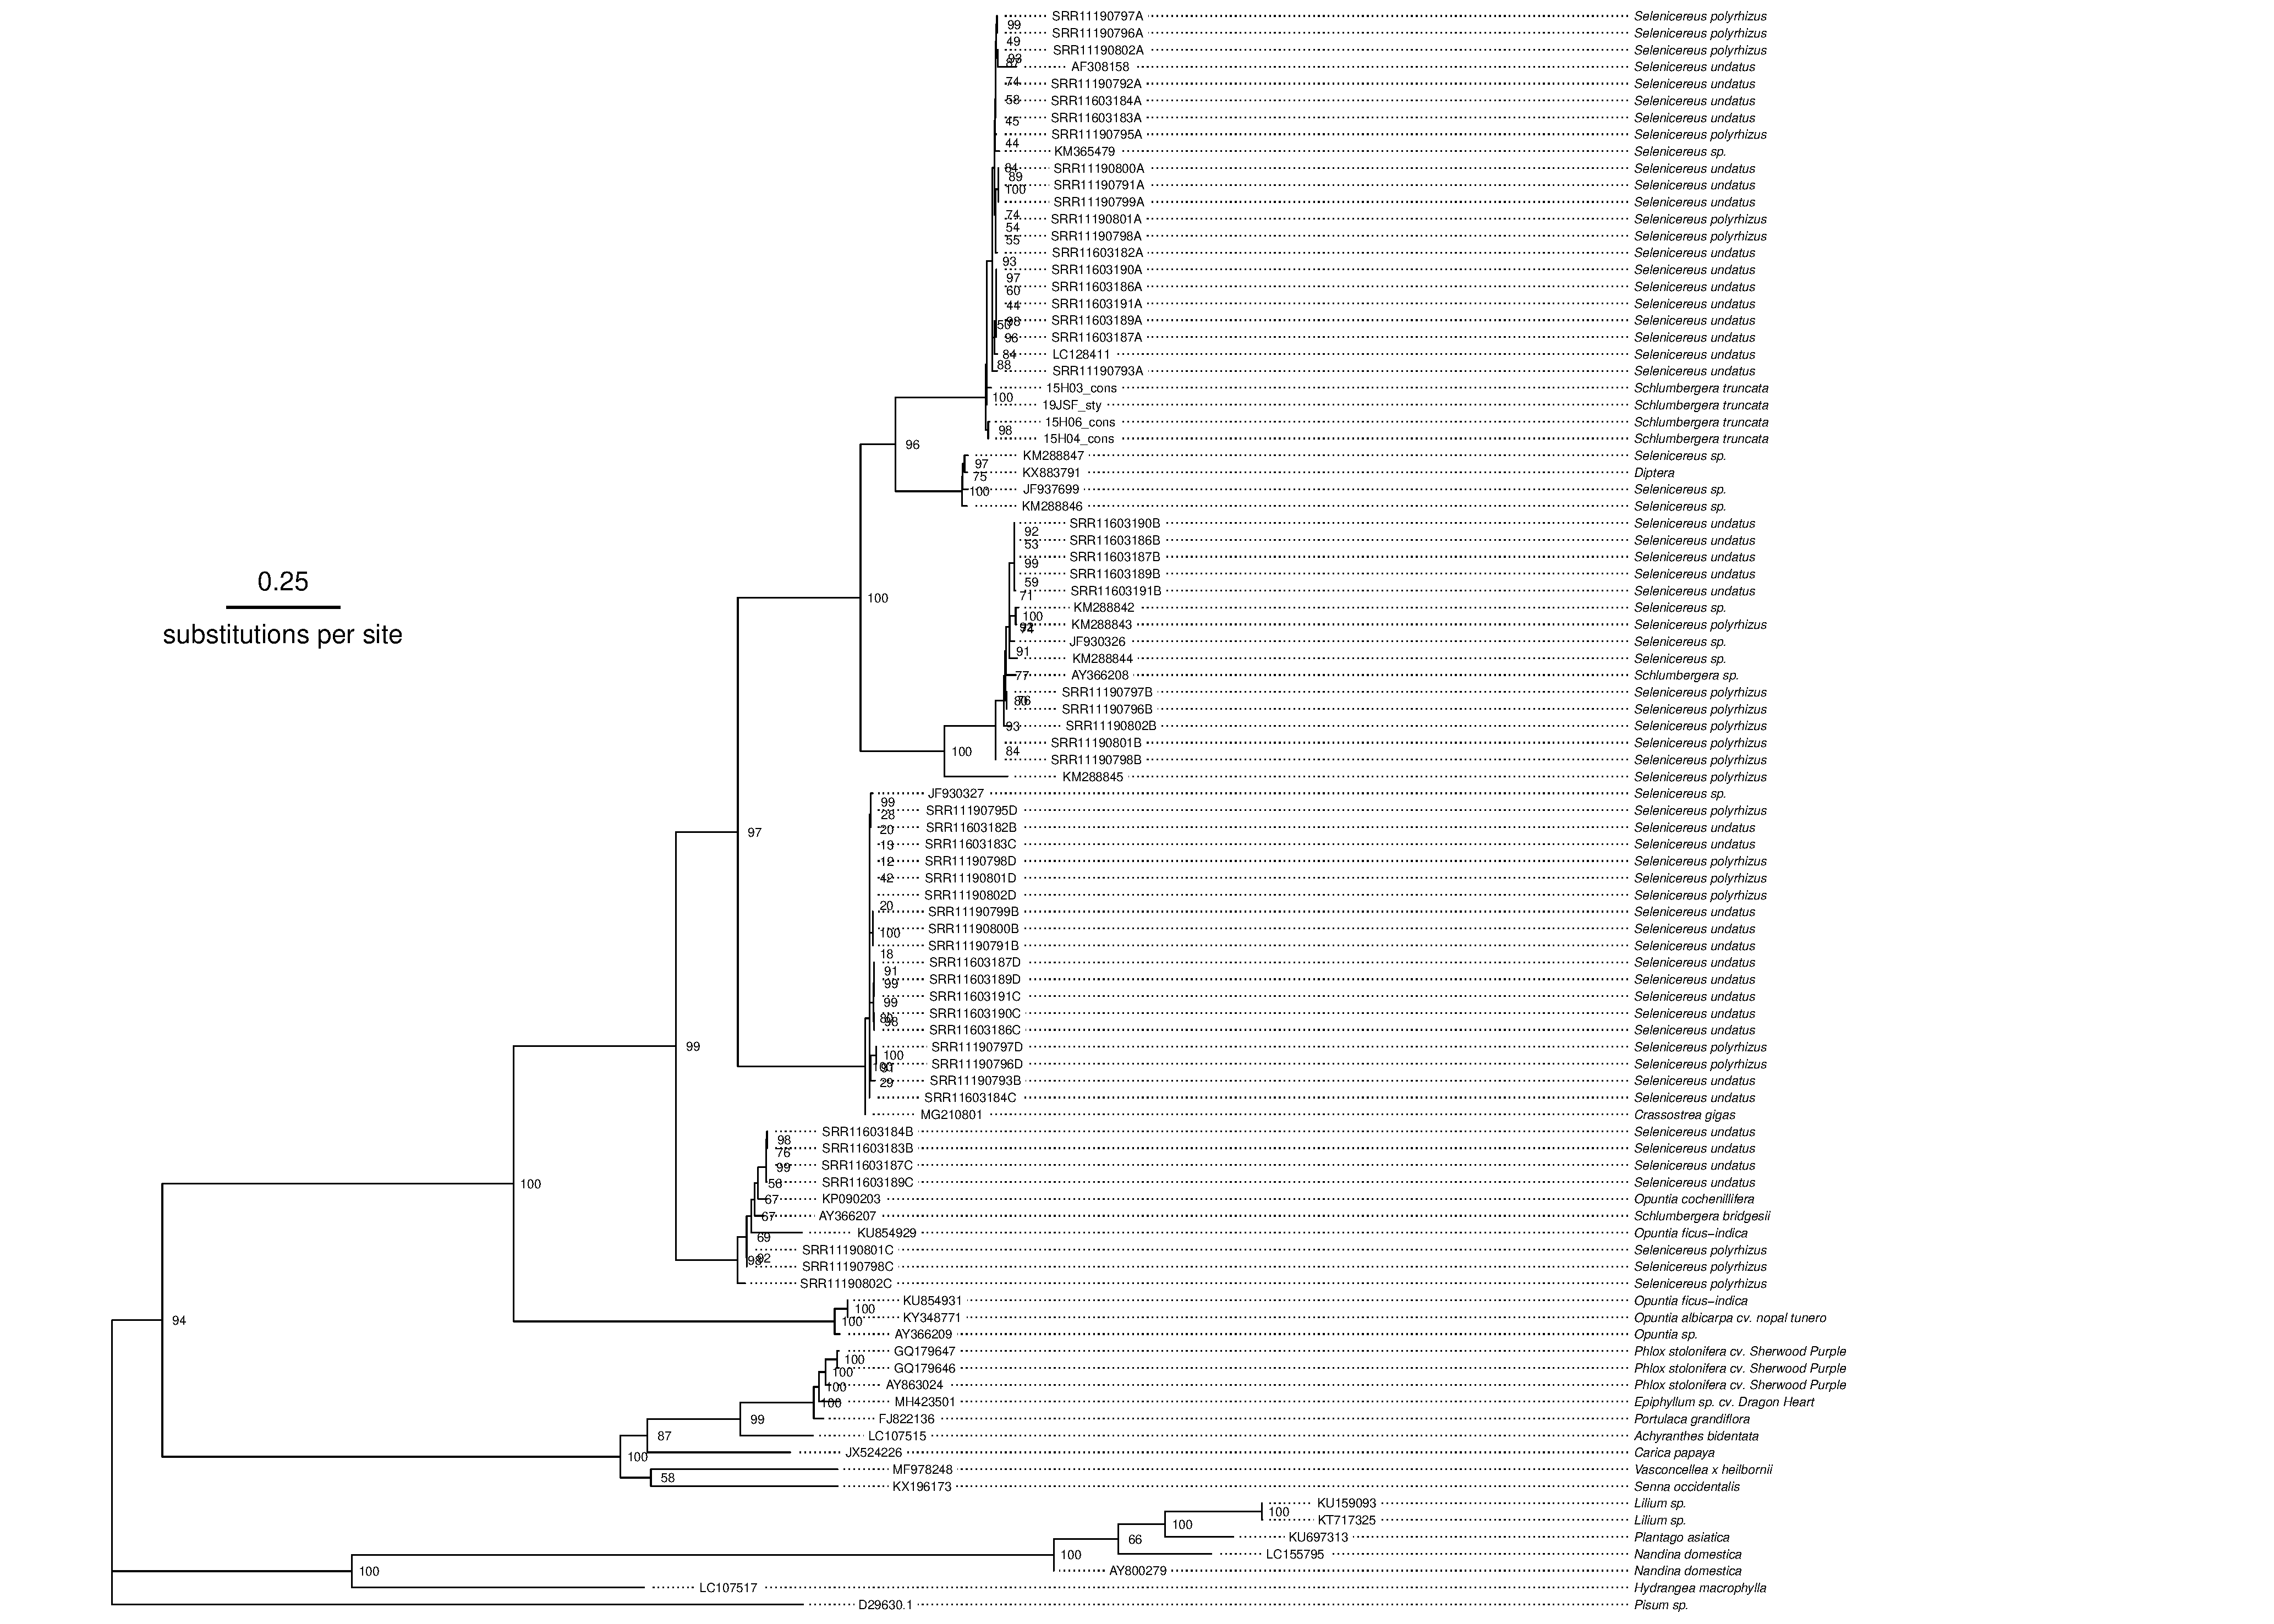
\includegraphics[width=1.3\textwidth]{supplementaryinfo/cp_tr.pdf}
\label{fig:genetree5}
\end{suppfigure}
\clearpage


%The support values are posterior probabilities of the respective
%delimitations, that is that the split defined by the respective branch
%splits the tree into two distinct species.
%
%The Bayesian version samples alternative delimitations.
%
%So the blue and red colors show you the most plausible delimitation into
%species and individuals from the same species.

%Fig S6:  mPTP tree
\begin{suppfigure}
\centering
\caption{
mPTP whole genome tree with delimitation represented by green and red coloration. Green branches represent delimitation outside of clades and red branches represent delimitation inside of clades.
}
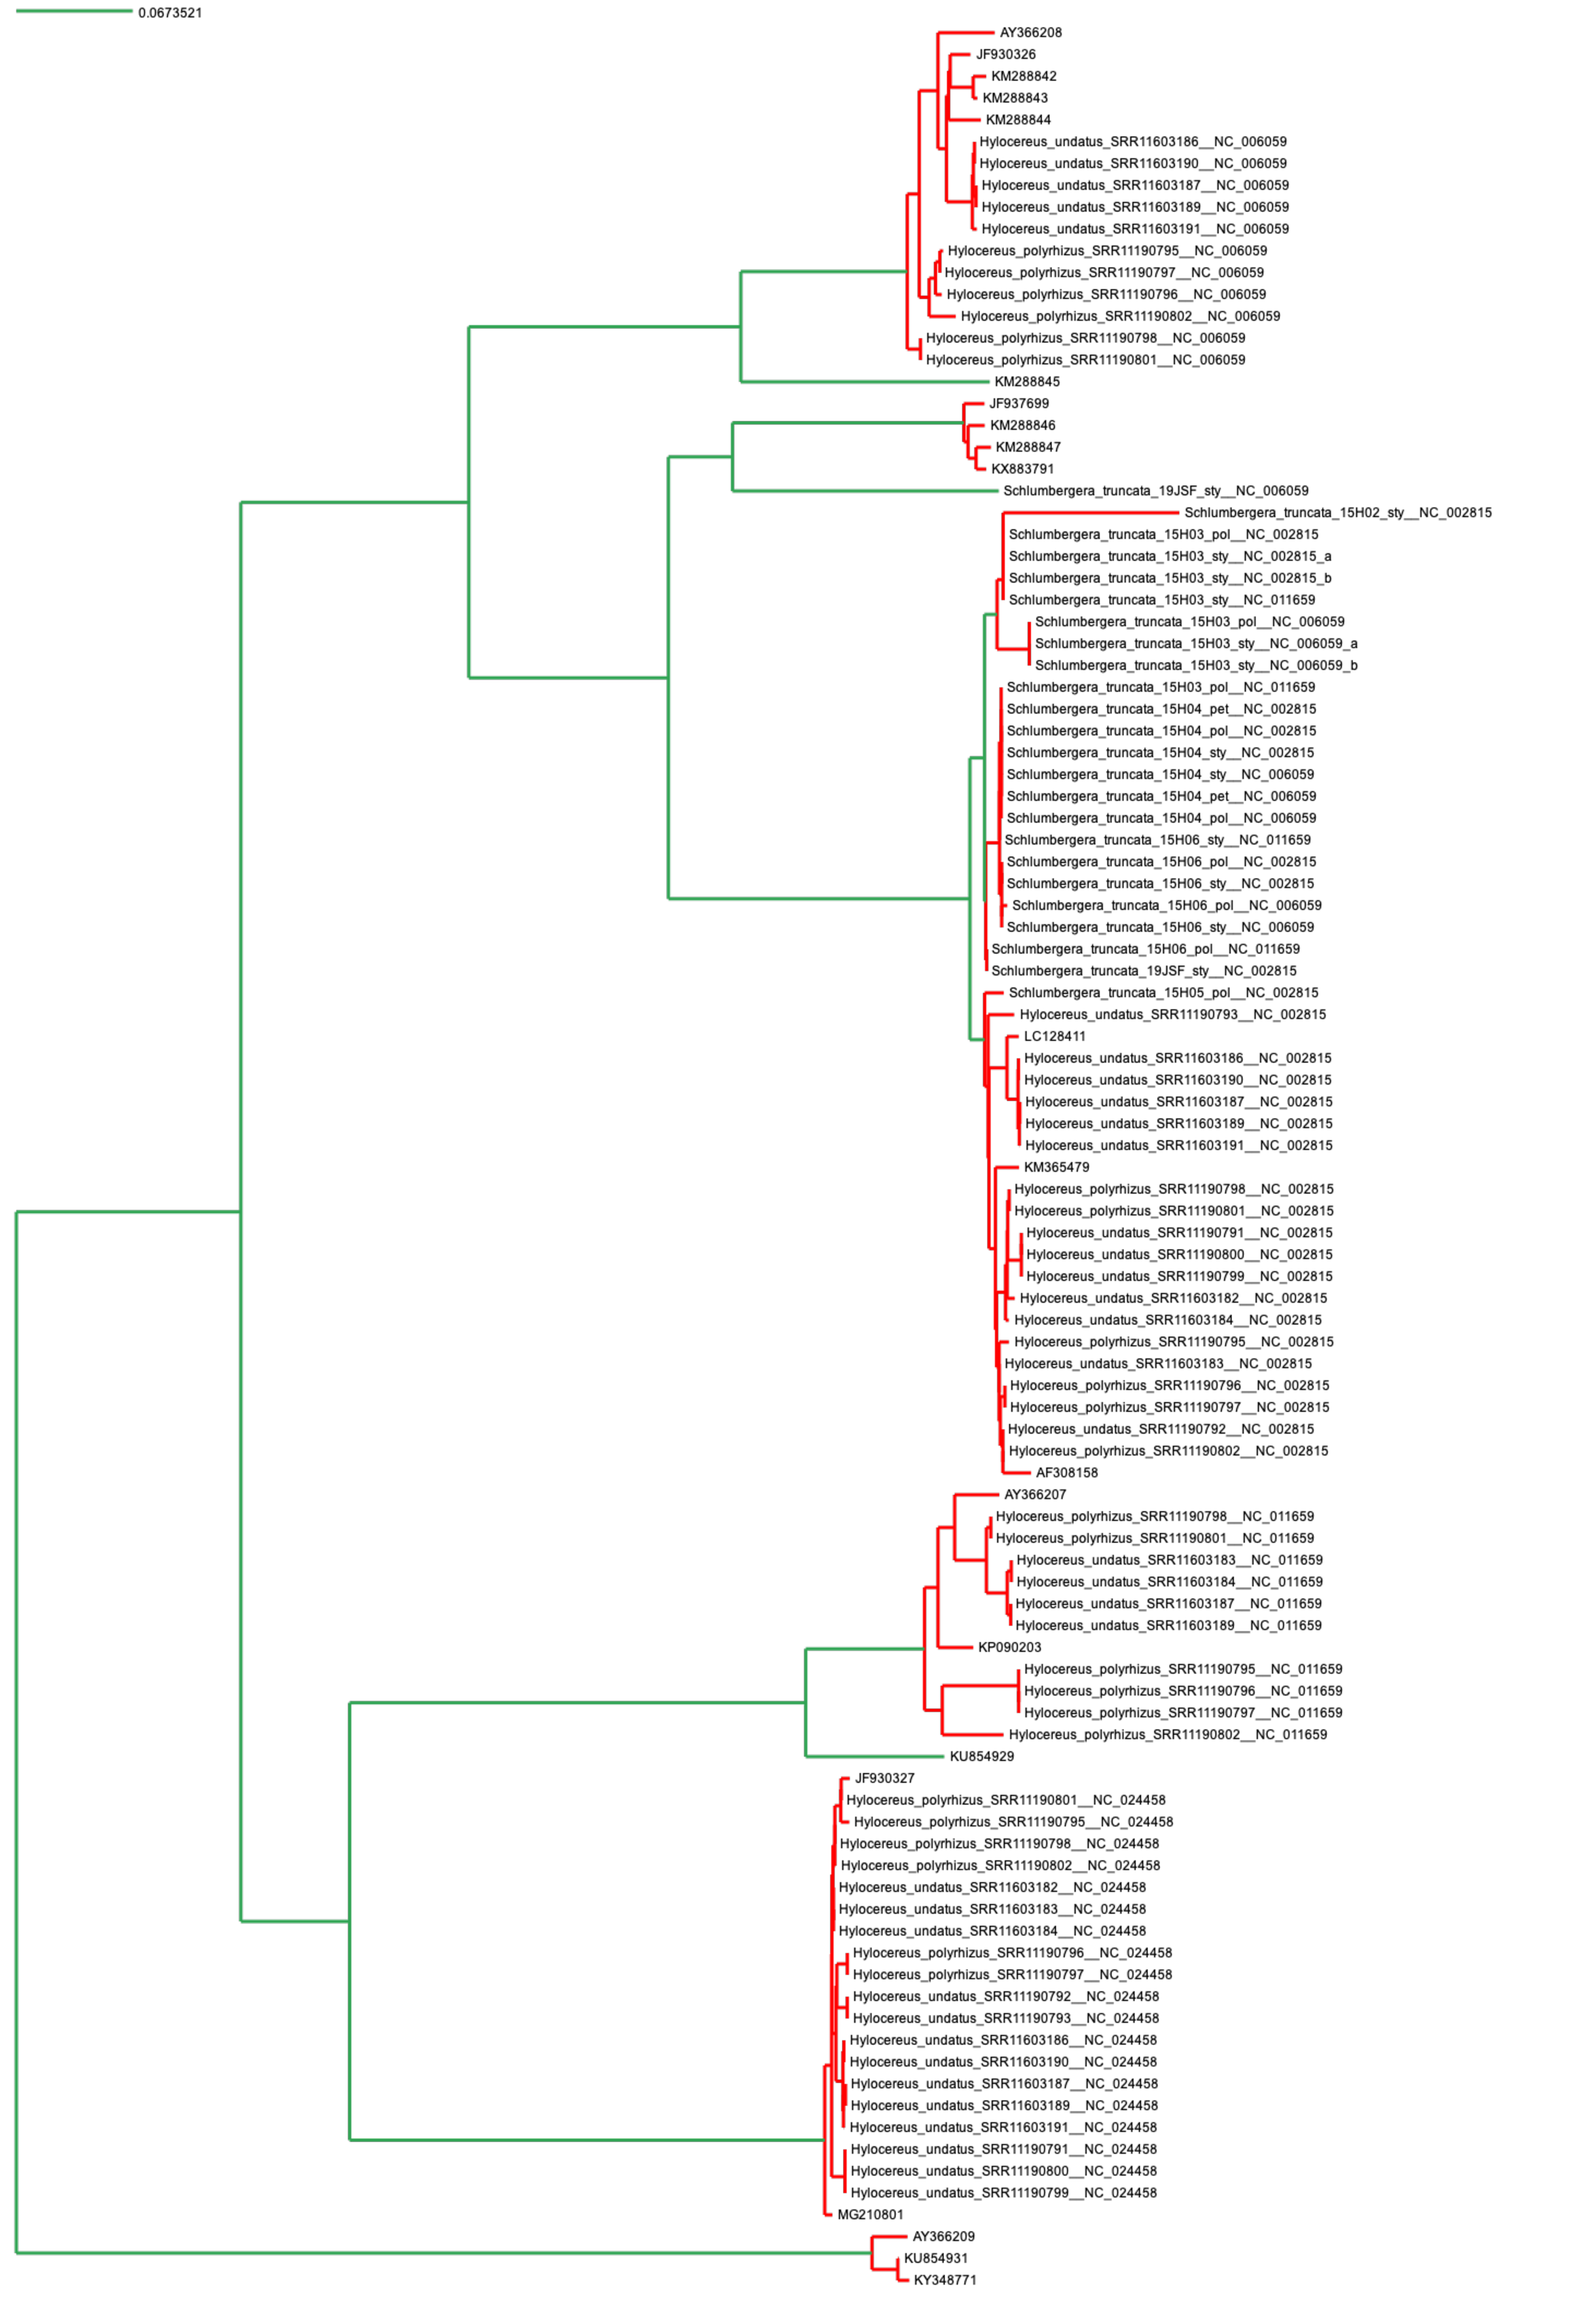
\includegraphics[width=0.8\textwidth]{supplementaryinfo/mptp.pdf}
\label{fig:genetree5}
\end{suppfigure}
\clearpage

%Fig S6:  bPTP tree
\begin{suppfigure}
\centering
\caption{
bPTP whole genome tree with delimitation represented by blue and red coloration. Numbers on nodes represent the posterior probability of the delimitation.
}
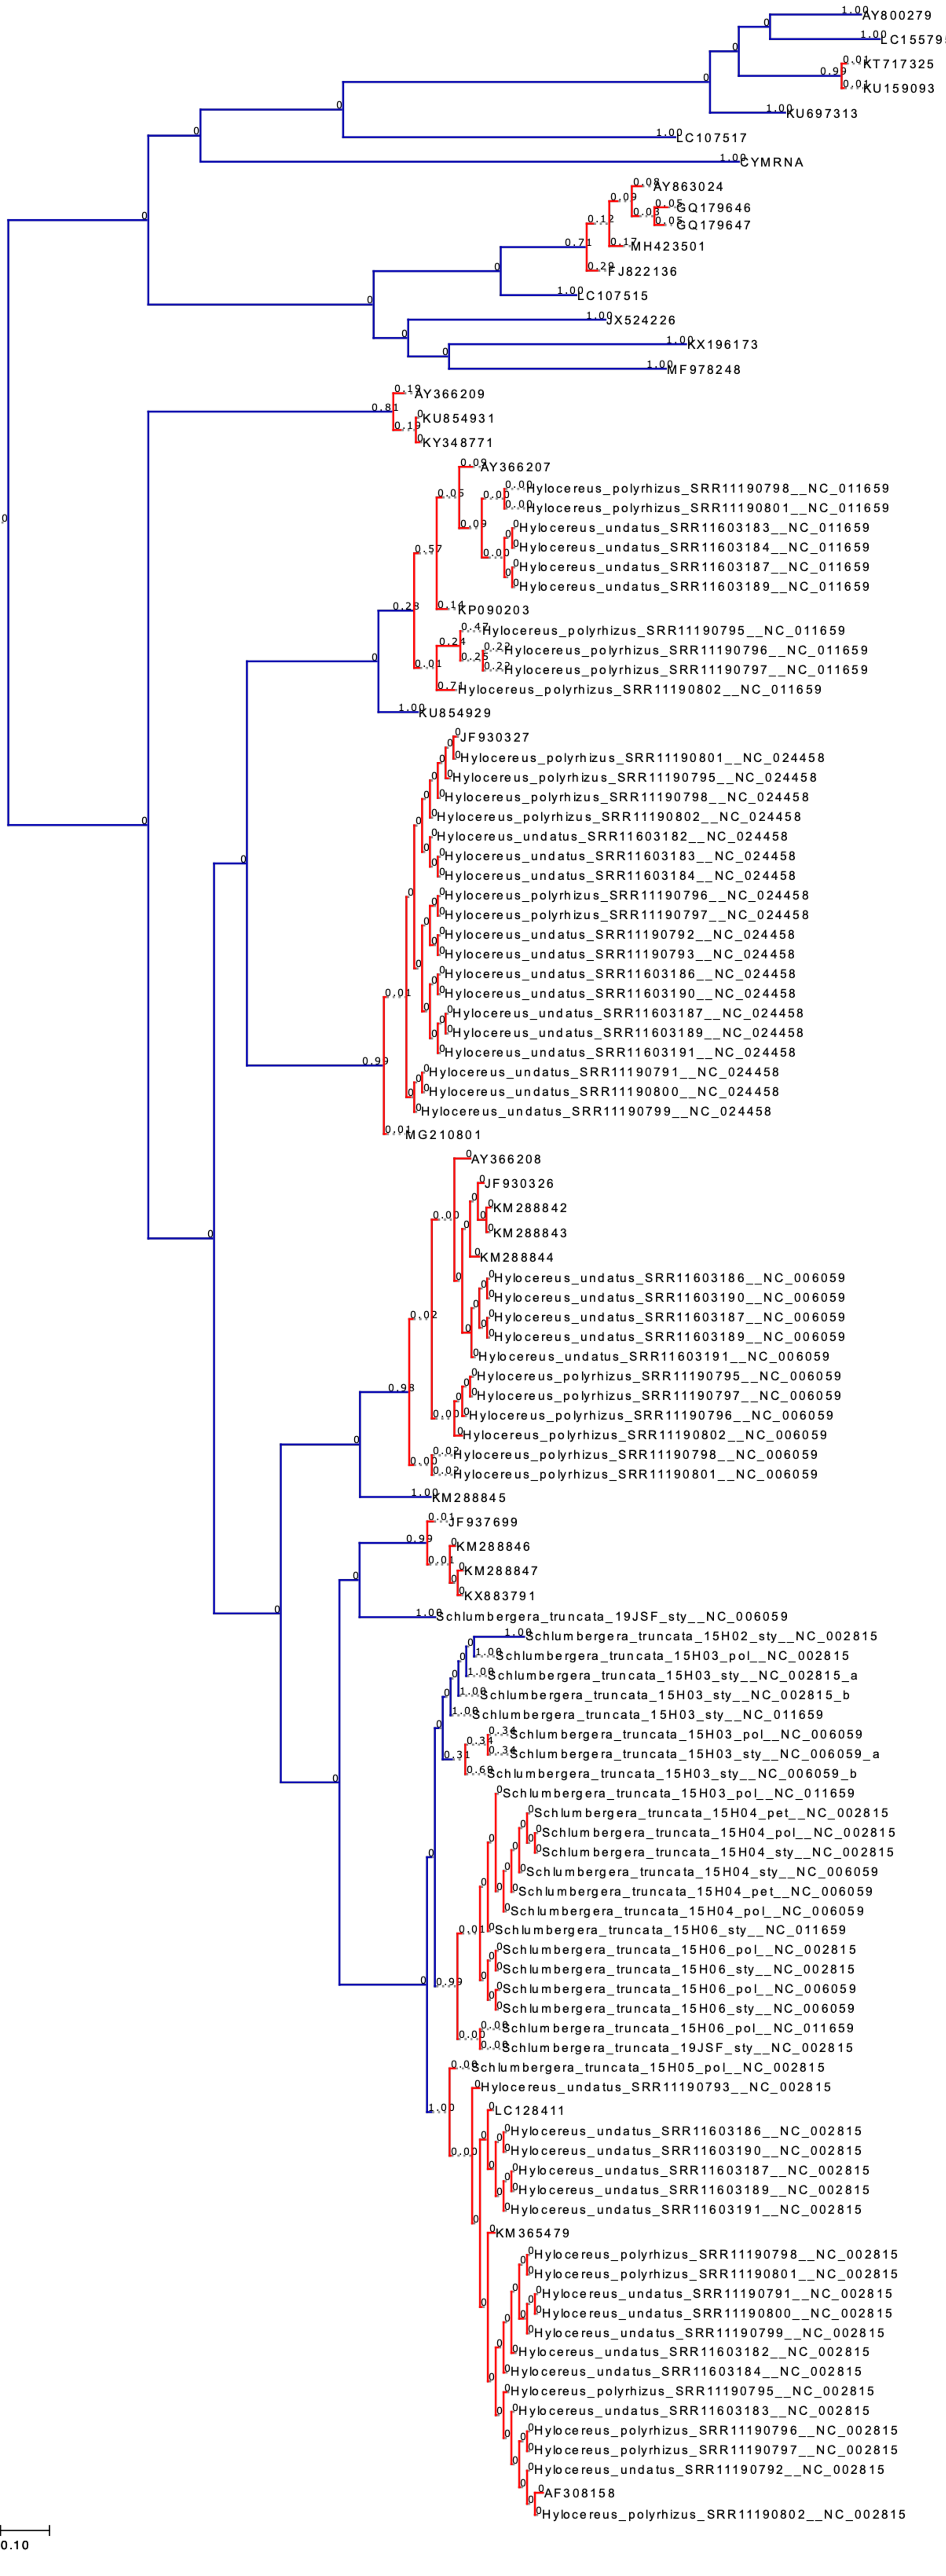
\includegraphics[width=0.4\textwidth]{supplementaryinfo/bptp.pdf}
\label{fig:genetree5}
\end{suppfigure}
\clearpage

%Fig S8:  bPTP; mPTP compared to formal tax
\begin{suppfigure}
\centering
\caption{
Visual demonstration of the agreement and disagreement of formal taxonomy, mPTP and bPTP delimitation methods as applied to the whole genome tree.
}
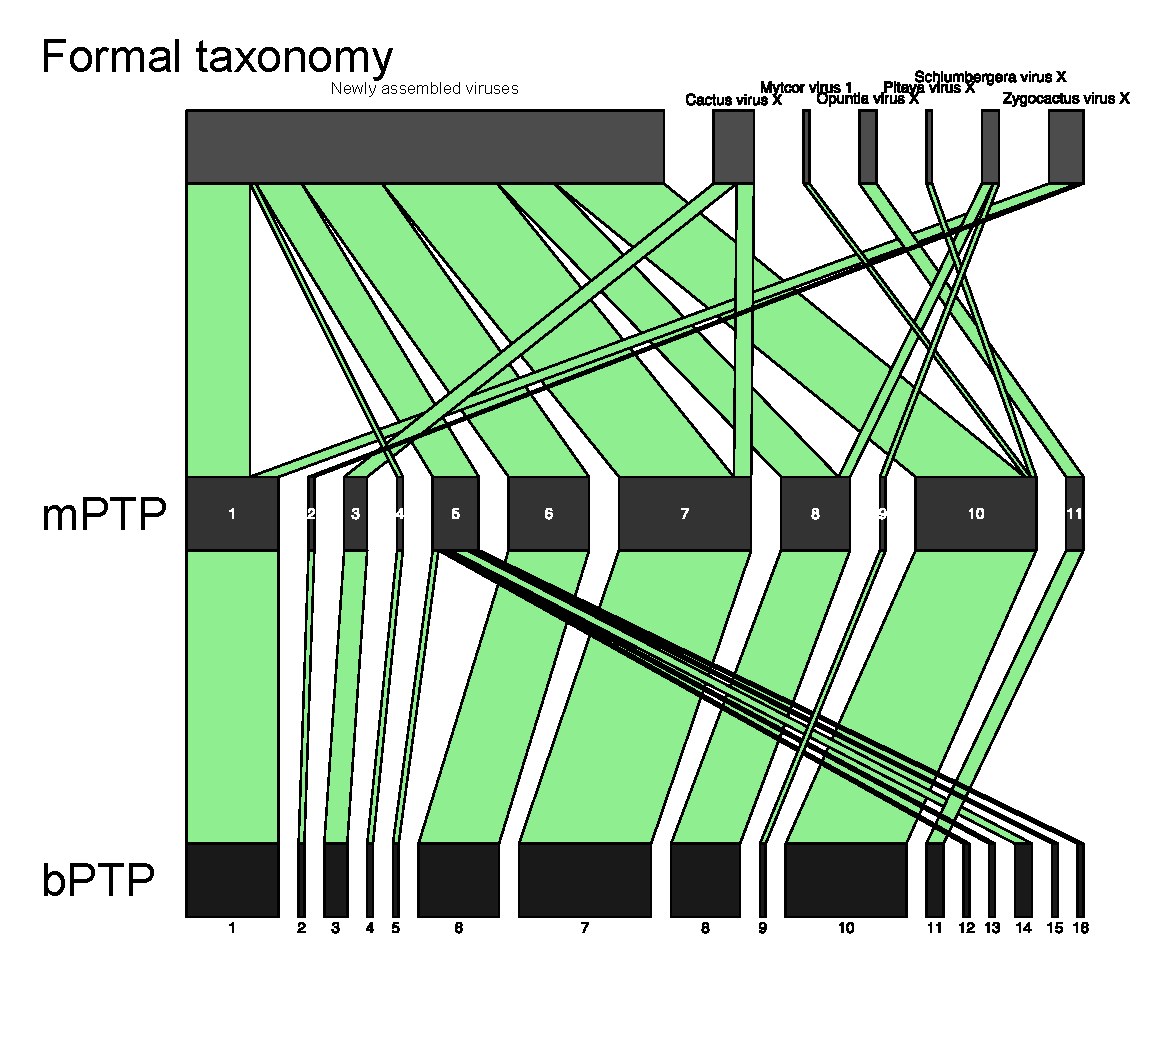
\includegraphics[width=0.8\textwidth]{supplementaryinfo/bipartite_web-edited.pdf}
\label{fig:genetree5}
\end{suppfigure}
\clearpage


%Fig S9:  bPTP; mPTP compared to each other
\begin{suppfigure}
\centering
\caption{
Bipartite graph displaying the disagreements between mPTP and bPTP methods. The main disagreement is located in clade 5 of mPTP, which is delimited into 7 separate species when bPTP methods are applied to the same data set.
}
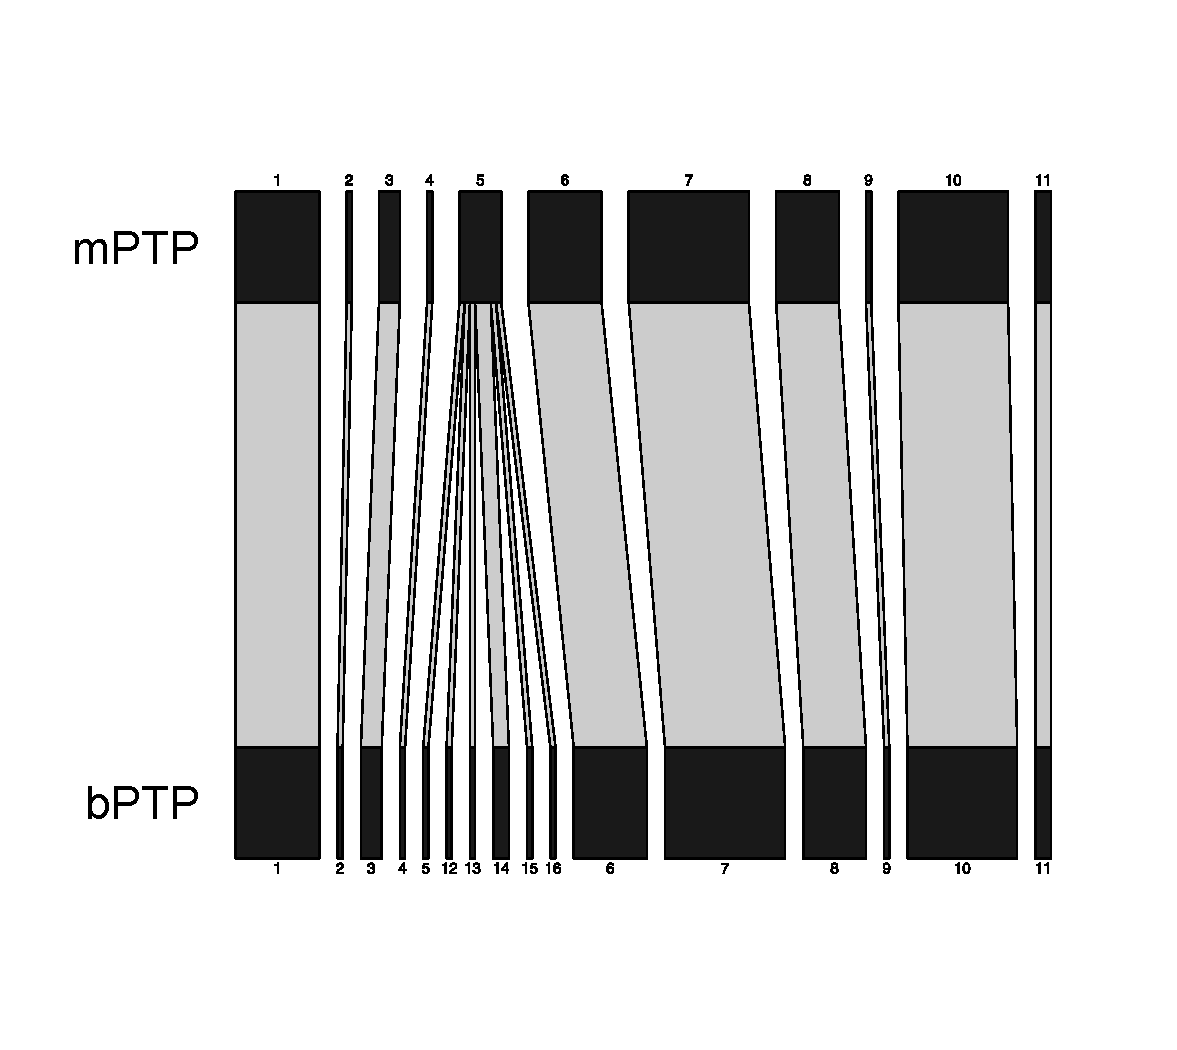
\includegraphics[width=0.8\textwidth]{supplementaryinfo/web.mPTP.bPTP-edited.pdf}
\label{fig:genetree5}
\end{suppfigure}
\clearpage
%
% TABLES
%S1: RNA-seq and assembly stats
%S2: Genbank stats
\begin{supptable}[ht]
\centering
\caption{RNA-seq and assembly summary statistics.
The length of all reads before trimming was 150 bp.
Column labelled \textsuperscript{*}filt. lists numbers of read pairs and average qualities after filtering step.} %FIXME: missing most of the caption.
% To browse your data, use SRA RunSelector:
% https://www.ncbi.nlm.nih.gov/Traces/study/?acc=PRJNA705387
% To see your summary list view (availability at this link subject to 24 hour delay):
% https://www.ncbi.nlm.nih.gov/sra/?term=PRJNA705387
\label{tab:suppSeqAsmbStats}
\resizebox{\textwidth}{!}{
\begin{tabular}{l|cc|cc|cc|cc|cc|c}
\toprule
\multicolumn{1}{c|}{} &
\multicolumn{2}{c|}{Read~pairs} &
\multicolumn{2}{c|}{Avg.~read~len.~trimmed} &
\multicolumn{2}{c|}{Avg.~qual.} &
\multicolumn{2}{c|}{Avg.~qual.~\textsuperscript{*}filt.} &
\multicolumn{2}{c|}{Assembly} &
\multicolumn{1}{c}{} \\
\multicolumn{1}{c|}{Sample} & Raw & \textsuperscript{*}filt. & F & R & F & R & F & R & Isoforms & Genes & SRR \\
\midrule
\textit{Schlumbergera truncata} 15H01 pol   & 4,841,466 & 3,353,072 & 149 & 147 & 35.8 & 34.8 & 36.2 & 35.8 & 43,294 & 27,125 & \href{https://trace.ncbi.nlm.nih.gov/Traces/sra/?run=SRR13805650}{SRR13805650} \\
\textit{Schlumbergera truncata} 15H01 sty   & 6,769,308 & 4,628,401 & 148 & 139 & 38.8 & 35.9 & 39.9 & 38.8 & 73,047 & 42,717 & \href{https://trace.ncbi.nlm.nih.gov/Traces/sra/?run=SRR13805653}{SRR13805653} \\
\textit{Schlumbergera truncata} 15H02 pol   & 4,888,079 & 3,353,774 & 149 & 147 & 35.8 & 35.0 & 36.2 & 35.8 & 48,134 & 30,138 & \href{https://trace.ncbi.nlm.nih.gov/Traces/sra/?run=SRR13805649}{SRR13805649} \\
\textit{Schlumbergera truncata} 15H02 sty   & 6,173,982 & 4,263,304 & 147 & 139 & 38.8 & 36.3 & 39.8 & 38.8 & 56,416 & 32,918 & \href{https://trace.ncbi.nlm.nih.gov/Traces/sra/?run=SRR13805652}{SRR13805652} \\
\textit{Schlumbergera truncata} 15H03 pol   & 6,983,951 & 4,858,975 & 149 & 147 & 35.8 & 35.1 & 36.2 & 35.9 & 53,675 & 32,640 & \href{https://trace.ncbi.nlm.nih.gov/Traces/sra/?run=SRR13805648}{SRR13805648} \\
\textit{Schlumbergera truncata} 15H03 sty 1 & 9,183,100 & 5,450,149 & 147 & 139 & 38.4 & 35.9 & 39.6 & 38.6 & 59,668 & 34,275 & \href{https://trace.ncbi.nlm.nih.gov/Traces/sra/?run=SRR13805641}{SRR13805641} \\
\textit{Schlumbergera truncata} 15H03 sty 2 & 7,147,068 & 4,815,235 & 148 & 139 & 38.7 & 36.1 & 39.8 & 38.7 & 48,708 & 28,407 & \href{https://trace.ncbi.nlm.nih.gov/Traces/sra/?run=SRR13805637}{SRR13805637} \\
\textit{Schlumbergera truncata} 15H04 pol   & 8,392,597 & 5,497,308 & 148 & 138 & 38.8 & 35.8 & 39.8 & 38.6 & 58,662 & 35,689 & \href{https://trace.ncbi.nlm.nih.gov/Traces/sra/?run=SRR13805647}{SRR13805647} \\
\textit{Schlumbergera truncata} 15H04 sty   & 5,240,352 & 3,446,465 & 147 & 140 & 38.6 & 36.4 & 39.8 & 38.8 & 54,120 & 31,872 & \href{https://trace.ncbi.nlm.nih.gov/Traces/sra/?run=SRR13805636}{SRR13805636} \\
\textit{Schlumbergera truncata} 15H05 pol   & 6,347,070 & 4,365,031 & 148 & 139 & 38.8 & 35.9 & 39.8 & 38.8 & 46,638 & 28,580 & \href{https://trace.ncbi.nlm.nih.gov/Traces/sra/?run=SRR13805646}{SRR13805646} \\
\textit{Schlumbergera truncata} 15H05 sty 1 & 9,618,084 & 6,479,817 & 146 & 139 & 38.2 & 35.9 & 39.6 & 38.8 & 71,031 & 41,443 & \href{https://trace.ncbi.nlm.nih.gov/Traces/sra/?run=SRR13805635}{SRR13805635} \\
\textit{Schlumbergera truncata} 15H05 sty 2 & 5,043,649 & 3,051,699 & 147 & 141 & 38.7 & 36.8 & 39.9 & 39.0 & 59,857 & 36,264 & \href{https://trace.ncbi.nlm.nih.gov/Traces/sra/?run=SRR13805634}{SRR13805634} \\
\textit{Schlumbergera truncata} 15H06 pol   & 6,850,087 & 4,360,475 & 148 & 141 & 38.9 & 36.5 & 39.7 & 38.8 & 27,729 & 18,571 & \href{https://trace.ncbi.nlm.nih.gov/Traces/sra/?run=SRR13805645}{SRR13805645} \\
\textit{Schlumbergera truncata} 15H06 sty   & 6,632,382 & 4,203,598 & 148 & 139 & 38.8 & 36.1 & 39.7 & 38.6 & 24,392 & 16,949 & \href{https://trace.ncbi.nlm.nih.gov/Traces/sra/?run=SRR13805633}{SRR13805633} \\
\textit{Schlumbergera truncata} 15H07 pol   & 4,513,581 & 2,988,451 & 148 & 147 & 35.7 & 35.0 & 36.2 & 35.9 & 46,908 & 29,464 & \href{https://trace.ncbi.nlm.nih.gov/Traces/sra/?run=SRR13805644}{SRR13805644} \\
\textit{Schlumbergera truncata} 15H07 sty   & 6,411,850 & 4,200,344 & 148 & 139 & 38.9 & 35.9 & 39.9 & 38.6 & 68,107 & 39,657 & \href{https://trace.ncbi.nlm.nih.gov/Traces/sra/?run=SRR13805632}{SRR13805632} \\
\textit{Schlumbergera truncata} 15H08 pol   & 5,106,699 & 3,863,997 & 149 & 147 & 35.8 & 35.1 & 36.2 & 35.8 & 36,739 & 23,618 & \href{https://trace.ncbi.nlm.nih.gov/Traces/sra/?run=SRR13805643}{SRR13805643} \\
\textit{Schlumbergera truncata} 15H08 sty   & 4,521,102 & 2,741,695 & 148 & 146 & 35.7 & 34.8 & 36.2 & 35.8 & 47,754 & 29,812 & \href{https://trace.ncbi.nlm.nih.gov/Traces/sra/?run=SRR13805631}{SRR13805631} \\
\textit{Schlumbergera truncata} 15H09 pol   & 4,645,325 & 2,575,494 & 148 & 147 & 35.7 & 35.0 & 36.2 & 35.8 & 42,245 & 27,650 & \href{https://trace.ncbi.nlm.nih.gov/Traces/sra/?run=SRR13805642}{SRR13805642} \\
\textit{Schlumbergera truncata} 15H09 root  & 6,653,640 & 3,261,445 & 149 & 148 & 35.7 & 34.4 & 36.4 & 36.2 & 68,427 & 48,463 & \href{https://trace.ncbi.nlm.nih.gov/Traces/sra/?run=SRR13805640}{SRR13805640} \\
\textit{Schlumbergera truncata} 15H09 stem  & 8,275,870 & 5,731,805 & 149 & 149 & 35.8 & 35.2 & 36.4 & 36.2 & 79,859 & 51,788 & \href{https://trace.ncbi.nlm.nih.gov/Traces/sra/?run=SRR13805639}{SRR13805639} \\
\textit{Schlumbergera truncata} 15H09 sty   & 6,363,556 & 4,525,356 & 147 & 138 & 38.8 & 35.8 & 39.8 & 38.7 & 62,991 & 36,275 & \href{https://trace.ncbi.nlm.nih.gov/Traces/sra/?run=SRR13805651}{SRR13805651} \\
\textit{Matucana madisoniorum} HBG13 sty    & 4,148,932 & 2,396,890 & 145 & 140 & 38.1 & 36.4 & 39.5 & 38.9 & 41,968 & 33,810 & \href{https://trace.ncbi.nlm.nih.gov/Traces/sra/?run=SRR13805638}{SRR13805638} \\
\bottomrule
\end{tabular}}
\end{supptable}



% Please add the following required packages to your document preamble:
% \usepackage{booktabs}
% \usepackage{graphicx}
% \usepackage[normalem]{ulem}
% \useunder{\uline}{\ul}{}
\begin{supptable}[ht]
\caption{
Genomes and gene sequences downloaded from the NCBI GenBank genome browser, descriptions of the genome, and associated hosts. 
}
\resizebox{2in}{!}{%
\rotatebox{90}{\begin{tabular}{@{}llllllll@{}}
\toprule
Name     & Accession  & Created Date                 & Description                                                                                                                                                                                                                                                      & Organism                       & Sequence Length & Size  & host                                  \\ \midrule
AF308158 & AF308158.2 & Mon Jul 02 00:00:00 CDT 2001 & Cactus virus X, complete genome                                                                                                                                                                                                                                  & Cactus virus X                 & 6614            & 21 KB & Selenicereus undatus                    \\
AY366207 & AY366207.2 & Fri Apr 23 00:00:00 CDT 2004 & Schlumbergera virus X strain K11, complete genome                                                                                                                                                                                                                & Schlumbergera virus X          & 6633            & 19 KB &                                       \\
AY366208 & AY366208.1 & Fri Apr 23 00:00:00 CDT 2004 & Zygocactus virus X strain B1 replication-associated protein, triple gene block protein 1, triple gene block protein 2, triple gene block protein 3, and coat protein genes, complete cds                                                                         & Zygocactus virus X             & 6624            & 18 KB &                                       \\
AY366209 & AY366209.1 & Fri Apr 23 00:00:00 CDT 2004 & Opuntia virus X strain CC10 replication-associated protein, triple gene block protein 1, triple gene block protein 2, triple gene block protein 3, and coat protein genes, complete cds                                                                          & Opuntia virus X                & 6653            & 18 KB &                                       \\
AY800279 & AY800279.1 & Fri Jul 01 00:00:00 CDT 2005 & Nandina mosaic virus isolate PLH 1, complete genome                                                                                                                                                                                                              & Nandina mosaic virus           & 6066            & 16 KB &                                       \\
AY863024 & AY863024.1 & Fri Dec 23 00:00:00 CST 2005 & Alternanthera mosaic virus, complete genome                                                                                                                                                                                                                      & Alternanthera mosaic virus     & 6607            & 26 KB & Phlox stolonifera cv. Sherwood Purple \\
CYMRNA   & D29630.1   & Fri Mar 25 00:00:00 CST 1994 & Clover yellow mosaic virus genomic RNA, complete sequence                                                                                                                                                                                                        & Clover yellow mosaic virus     & 7015            & 11 KB &                                       \\
FJ822136 & FJ822136.1 & Sun Apr 05 00:00:00 CDT 2009 & Alternanthera mosaic virus from Portulaca grandiflora, complete genome                                                                                                                                                                                           & Alternanthera mosaic virus     & 6606            & 21 KB & Portulaca grandiflora                 \\
GQ179646 & GQ179646.1 & Wed Sep 16 00:00:00 CDT 2009 & Alternanthera mosaic virus isolate SP 3-1, complete genome                                                                                                                                                                                                       & Alternanthera mosaic virus     & 6607            & 19 KB & Phlox stolonifera cv. Sherwood Purple \\
GQ179647 & GQ179647.1 & Wed Sep 16 00:00:00 CDT 2009 & Alternanthera mosaic virus isolate SP 4-7, complete genome                                                                                                                                                                                                       & Alternanthera mosaic virus     & 6607            & 19 KB & Phlox stolonifera cv. Sherwood Purple \\
JF930326 & JF930326.1 & Tue Jul 01 00:00:00 CDT 2014 & Zygocactus virus X isolate P39, complete genome                                                                                                                                                                                                                  & Zygocactus virus X             & 6624            & 18 KB & Selenicereus sp.                        \\
JF930327 & JF930327.1 & Tue Jul 01 00:00:00 CDT 2014 & Pitaya virus X isolate P37, complete genome                                                                                                                                                                                                                      & Pitaya virus X                 & 6677            & 18 KB & Selenicereus sp.                        \\
JF937699 & JF937699.1 & Tue Jul 01 00:00:00 CDT 2014 & Cactus virus X isolate NTU, complete genome                                                                                                                                                                                                                      & Cactus virus X                 & 6627            & 18 KB & Selenicereus sp.                        \\
JX524226 & JX524226.1 & Sun Oct 28 00:00:00 CDT 2012 & Papaya mosaic virus isolate PMV-HN, complete genome                                                                                                                                                                                                              & Papaya mosaic virus            & 6656            & 19 KB & Carica papaya                         \\
KM288842 & KM288842.1 & Fri Sep 30 00:00:00 CDT 2016 & Zygocactus virus X isolate TW-4XB-2 replication-associated protein (RdRP) gene, partial cds; and triple gene block protein 1 (TGB1), triple gene block protein 2 (TGB2), triple gene block protein 3 (TGB3), and coat protein (CP) genes, complete cds           & Zygocactus virus X             & 2403            & 15 KB & Selenicereus sp. (pitaya)               \\
KM288843 & KM288843.1 & Fri Sep 30 00:00:00 CDT 2016 & Zygocactus virus X isolate TW-456Y-4 triple gene block protein 1 (TGB1) gene, partial cds; and triple gene block protein 2 (TGB2), triple gene block protein 3 (TGB3), and coat protein (CP) genes, complete cds                                                 & Zygocactus virus X             & 1671            & 13 KB & Selenicereus sp. (pitaya)               \\
KM288844 & KM288844.1 & Fri Sep 30 00:00:00 CDT 2016 & Zygocactus virus X isolate TW-5149-5 replication-associated protein (RdRP) gene, partial cds; and triple gene block protein 1 (TGB1), triple gene block protein 2 (TGB2), triple gene block protein 3 (TGB3), and coat protein (CP) genes, complete cds          & Zygocactus virus X             & 2399            & 16 KB & Selenicereus sp. (pitaya)               \\
KM288845 & KM288845.1 & Fri Sep 30 00:00:00 CDT 2016 & Zygocactus virus X isolate TW-5149-17 replication-associated protein (RdRP) gene, partial cds; and triple gene block protein 1 (TGB1), triple gene block protein 2 (TGB2), triple gene block protein 3 (TGB3), and coat protein (CP) genes, complete cds         & Zygocactus virus X             & 2397            & 16 KB & Selenicereus sp. (pitaya)               \\
KM288846 & KM288846.1 & Fri Sep 30 00:00:00 CDT 2016 & Cactus virus X isolate TW-5XB-1 replication-associated protein (RdRP) gene, partial cds; and triple gene block protein 1 (TGB1), triple gene block protein 2 (TGB2), triple gene block protein 3 (TGB3), and coat protein (CP) genes, complete cds               & Cactus virus X                 & 2418            & 16 KB & Selenicereus sp. (pitaya)               \\
KM288847 & KM288847.1 & Fri Sep 30 00:00:00 CDT 2016 & Cactus virus X isolate TW-456Y-1 triple gene block protein 1 (TGB1) gene, partial cds; and triple gene block protein 2 (TGB2), triple gene block protein 3 (TGB3), and coat protein (CP) genes, complete cds                                                     & Cactus virus X                 & 1675            & 13 KB & Selenicereus sp. (pitaya)               \\
KM365479 & KM365479.1 & Mon Nov 17 00:00:00 CST 2014 & Cactus virus X isolate TW-5149-20 replication-associated protein (CVXgp1) gene, partial cds; and triple gene block protein 1 (CVXgp2), triple gene block protein 2 (CVXgp3), triple gene block protein 3 (CVXgp4), and coat protein (CVXgp5) genes, complete cds & Cactus virus X                 & 2396            & 15 KB & Selenicereus sp. (pitaya)               \\
KP090203 & KP090203.1 & Tue Jan 27 00:00:00 CST 2015 & Schlumbergera virus X isolate Palma-PE, complete genome                                                                                                                                                                                                          & Schlumbergera virus X          & 6615            & 20 KB & Opuntia cochenillifera                \\
KT717325 & KT717325.1 & Sat Feb 13 00:00:00 CST 2016 & Plantago asiatica mosaic virus isolate kr, complete genome                                                                                                                                                                                                       & Plantago asiatica mosaic virus & 6101            & 19 KB & Lilium sp.                            \\
KU159093 & KU159093.1 & Wed Apr 20 00:00:00 CDT 2016 & Plantago asiatica mosaic virus isolate Ko-YS, complete genome                                                                                                                                                                                                    & Plantago asiatica mosaic virus & 6102            & 17 KB & lily                                  \\
KU697313 & KU697313.1 & Mon Mar 07 00:00:00 CST 2016 & Plantago asiatica mosaic virus isolate Gunwi, complete genome                                                                                                                                                                                                    & Plantago asiatica mosaic virus & 6130            & 19 KB & Plantago asiatica                     \\
KU854929 & KU854929.1 & Tue May 31 00:00:00 CDT 2016 & Schlumbergera virus X isolate nopal verdura 1, complete genome                                                                                                                                                                                                   & Schlumbergera virus X          & 6646            & 21 KB & Opuntia ficus-indica                  \\
KU854931 & KU854931.1 & Tue May 31 00:00:00 CDT 2016 & Opuntia virus X isolate nopal verdura-1, complete genome                                                                                                                                                                                                         & Opuntia virus X                & 6667            & 21 KB & Opuntia ficus-indica                  \\
KX196173 & KX196173.2 & Sun Jul 31 00:00:00 CDT 2016 & Senna mosaic virus isolate Brazilian, complete genome                                                                                                                                                                                                            & Senna mosaic virus             & 6775            & 20 KB & Senna occidentalis                    \\
KX883791 & KX883791.1 & Sat Dec 10 00:00:00 CST 2016 & Cactus virus X strain SCM51431 ORF1, ORF2, ORF3, and ORF4 genes, complete cds                                                                                                                                                                                    & Cactus virus X                 & 6610            & 20 KB & Diptera                               \\
KY348771 & KY348771.1 & Mon Nov 13 00:00:00 CST 2017 & Opuntia virus X isolate Noptuna-Mex, complete genome                                                                                                                                                                                                             & Opuntia virus X                & 6656            & 20 KB & Opuntia albicarpa cv. nopal tunero    \\
LC107515 & LC107515.1 & Tue Feb 02 00:00:00 CST 2016 & Alternanthera mosaic virus genomic RNA, complete genome, isolate: Ac                                                                                                                                                                                             & Alternanthera mosaic virus     & 6604            & 21 KB & Achyranthes bidentata                 \\
LC107517 & LC107517.1 & Tue Feb 02 00:00:00 CST 2016 & Hydrangea ringspot virus genomic RNA, complete genome, isolate: Gu2                                                                                                                                                                                              & Hydrangea ringspot virus       & 6196            & 22 KB & Hydrangea macrophylla                 \\
LC128411 & LC128411.1 & Wed Mar 30 00:00:00 CDT 2016 & Cactus virus X genomic RNA, complete genome                                                                                                                                                                                                                      & Cactus virus X                 & 6618            & 19 KB & Selenicereus undatus                    \\
LC155795 & LC155795.1 & Fri Mar 24 00:00:00 CDT 2017 & Plantago asiatica mosaic virus genomic RNA, complete genome, isolate: NJ                                                                                                                                                                                         & Plantago asiatica mosaic virus & 6122            & 20 KB & Nandina domestica                     \\
MF978248 & MF978248.1 & Tue Dec 26 00:00:00 CST 2017 & Babaco mosaic virus isolate Tandapi, complete genome                                                                                                                                                                                                             & Babaco mosaic virus            & 6692            & 20 KB & Vasconcellea x heilbornii             \\
MG210801 & MG210801.1 & Tue Oct 30 00:00:00 CDT 2018 & Mytcor virus 1 replicative protein gene, partial cds; and protein 2 and protein 3 genes, complete cds                                                                                                                                                            & Mytcor virus 1                 & 5689            & 14 KB & Mytilus coruscus                      \\
MH423501 & MH423501.1 & Sun Feb 17 00:00:00 CST 2019 & Alternanthera mosaic virus isolate DH, complete genome                                                                                                                                                                                                           & Alternanthera mosaic virus     & 6598            & 18 KB & Epiphyllum sp. cv. Dragon Heart       \\ \bottomrule
\end{tabular}}%
}

\end{supptable}


\restoregeometry



% Please add the following required packages to your document preamble:
% \usepackage{booktabs}
% \usepackage{graphicx}
\begin{supptable}[ht]

\caption{
Assembled viral sequences from transcriptomes previously uploaded to GenBank. 
}
\resizebox{\textwidth}{!}{%
\begin{tabular}{@{}llllll@{}}
\toprule
Name                                              & sample\_name & Description\_mapped\_to & Sequence Length & Size & host                  \\ \midrule
Hylocereus\_polyrhizus\_SRR11190795\_\_NC\_002815 & SRR11190795  & NC\_002815              & 6614            & 7 KB & Selenicereus polyrhizus \\
Hylocereus\_polyrhizus\_SRR11190795\_\_NC\_006059 & SRR11190795  & NC\_006059              & 6624            & 7 KB & Selenicereus polyrhizus \\
Hylocereus\_polyrhizus\_SRR11190795\_\_NC\_011659 & SRR11190795  & NC\_011659              & 6633            & 7 KB & Selenicereus polyrhizus \\
Hylocereus\_polyrhizus\_SRR11190795\_\_NC\_024458 & SRR11190795  & NC\_024458              & 6677            & 7 KB & Selenicereus polyrhizus \\
Hylocereus\_polyrhizus\_SRR11190796\_\_NC\_002815 & SRR11190796  & NC\_002815              & 6614            & 7 KB & Selenicereus polyrhizus \\
Hylocereus\_polyrhizus\_SRR11190796\_\_NC\_006059 & SRR11190796  & NC\_006059              & 6624            & 7 KB & Selenicereus polyrhizus \\
Hylocereus\_polyrhizus\_SRR11190796\_\_NC\_011659 & SRR11190796  & NC\_011659              & 6633            & 7 KB & Selenicereus polyrhizus \\
Hylocereus\_polyrhizus\_SRR11190796\_\_NC\_024458 & SRR11190796  & NC\_024458              & 6677            & 7 KB & Selenicereus polyrhizus \\
Hylocereus\_polyrhizus\_SRR11190797\_\_NC\_002815 & SRR11190797  & NC\_002815              & 6614            & 7 KB & Selenicereus polyrhizus \\
Hylocereus\_polyrhizus\_SRR11190797\_\_NC\_006059 & SRR11190797  & NC\_006059              & 6624            & 7 KB & Selenicereus polyrhizus \\
Hylocereus\_polyrhizus\_SRR11190797\_\_NC\_011659 & SRR11190797  & NC\_011659              & 6633            & 7 KB & Selenicereus polyrhizus \\
Hylocereus\_polyrhizus\_SRR11190797\_\_NC\_024458 & SRR11190797  & NC\_024458              & 6677            & 7 KB & Selenicereus polyrhizus \\
Hylocereus\_polyrhizus\_SRR11190798\_\_NC\_002815 & SRR11190798  & NC\_002815              & 6614            & 7 KB & Selenicereus polyrhizus \\
Hylocereus\_polyrhizus\_SRR11190798\_\_NC\_006059 & SRR11190798  & NC\_006059              & 6624            & 7 KB & Selenicereus polyrhizus \\
Hylocereus\_polyrhizus\_SRR11190798\_\_NC\_011659 & SRR11190798  & NC\_011659              & 6633            & 7 KB & Selenicereus polyrhizus \\
Hylocereus\_polyrhizus\_SRR11190798\_\_NC\_024458 & SRR11190798  & NC\_024458              & 6677            & 7 KB & Selenicereus polyrhizus \\
Hylocereus\_polyrhizus\_SRR11190801\_\_NC\_002815 & SRR11190801  & NC\_002815              & 6614            & 7 KB & Selenicereus polyrhizus \\
Hylocereus\_polyrhizus\_SRR11190801\_\_NC\_006059 & SRR11190801  & NC\_006059              & 6624            & 7 KB & Selenicereus polyrhizus \\
Hylocereus\_polyrhizus\_SRR11190801\_\_NC\_011659 & SRR11190801  & NC\_011659              & 6633            & 7 KB & Selenicereus polyrhizus \\
Hylocereus\_polyrhizus\_SRR11190801\_\_NC\_024458 & SRR11190801  & NC\_024458              & 6677            & 7 KB & Selenicereus polyrhizus \\
Hylocereus\_polyrhizus\_SRR11190802\_\_NC\_002815 & SRR11190802  & NC\_002815              & 6614            & 7 KB & Selenicereus polyrhizus \\
Hylocereus\_polyrhizus\_SRR11190802\_\_NC\_006059 & SRR11190802  & NC\_006059              & 6624            & 7 KB & Selenicereus polyrhizus \\
Hylocereus\_polyrhizus\_SRR11190802\_\_NC\_011659 & SRR11190802  & NC\_011659              & 6633            & 7 KB & Selenicereus polyrhizus \\
Hylocereus\_polyrhizus\_SRR11190802\_\_NC\_024458 & SRR11190802  & NC\_024458              & 6677            & 7 KB & Selenicereus polyrhizus \\
Hylocereus\_undatus\_SRR11190791\_\_NC\_002815    & SRR11190791  & NC\_002815              & 6614            & 7 KB & Selenicereus undatus    \\
Hylocereus\_undatus\_SRR11190791\_\_NC\_024458    & SRR11190791  & NC\_024458              & 6677            & 7 KB & Selenicereus undatus    \\
Hylocereus\_undatus\_SRR11190792\_\_NC\_002815    & SRR11190792  & NC\_002815              & 6614            & 7 KB & Selenicereus undatus    \\
Hylocereus\_undatus\_SRR11190792\_\_NC\_024458    & SRR11190792  & NC\_024458              & 6677            & 7 KB & Selenicereus undatus    \\
Hylocereus\_undatus\_SRR11190793\_\_NC\_002815    & SRR11190793  & NC\_002815              & 6614            & 7 KB & Selenicereus undatus    \\
Hylocereus\_undatus\_SRR11190793\_\_NC\_024458    & SRR11190793  & NC\_024458              & 6677            & 7 KB & Selenicereus undatus    \\
Hylocereus\_undatus\_SRR11190799\_\_NC\_002815    & SRR11190799  & NC\_002815              & 6614            & 7 KB & Selenicereus undatus    \\
Hylocereus\_undatus\_SRR11190799\_\_NC\_024458    & SRR11190799  & NC\_024458              & 6677            & 7 KB & Selenicereus undatus    \\
Hylocereus\_undatus\_SRR11190800\_\_NC\_002815    & SRR11190800  & NC\_002815              & 6614            & 7 KB & Selenicereus undatus    \\
Hylocereus\_undatus\_SRR11190800\_\_NC\_024458    & SRR11190800  & NC\_024458              & 6677            & 7 KB & Selenicereus undatus    \\
Hylocereus\_undatus\_SRR11603182\_\_NC\_002815    & SRR11603182  & NC\_002815              & 6614            & 7 KB & Selenicereus undatus    \\
Hylocereus\_undatus\_SRR11603182\_\_NC\_024458    & SRR11603182  & NC\_024458              & 6677            & 7 KB & Selenicereus undatus    \\
Hylocereus\_undatus\_SRR11603183\_\_NC\_002815    & SRR11603183  & NC\_002815              & 6614            & 7 KB & Selenicereus undatus    \\
Hylocereus\_undatus\_SRR11603183\_\_NC\_011659    & SRR11603183  & NC\_011659              & 6633            & 7 KB & Selenicereus undatus    \\
Hylocereus\_undatus\_SRR11603183\_\_NC\_024458    & SRR11603183  & NC\_024458              & 6677            & 7 KB & Selenicereus undatus    \\
Hylocereus\_undatus\_SRR11603184\_\_NC\_002815    & SRR11603184  & NC\_002815              & 6614            & 7 KB & Selenicereus undatus    \\
Hylocereus\_undatus\_SRR11603184\_\_NC\_011659    & SRR11603184  & NC\_011659              & 6633            & 7 KB & Selenicereus undatus    \\
Hylocereus\_undatus\_SRR11603184\_\_NC\_024458    & SRR11603184  & NC\_024458              & 6677            & 7 KB & Selenicereus undatus    \\
Hylocereus\_undatus\_SRR11603186\_\_NC\_002815    & SRR11603186  & NC\_002815              & 6614            & 7 KB & Selenicereus undatus    \\
Hylocereus\_undatus\_SRR11603186\_\_NC\_006059    & SRR11603186  & NC\_006059              & 6624            & 7 KB & Selenicereus undatus    \\
Hylocereus\_undatus\_SRR11603186\_\_NC\_024458    & SRR11603186  & NC\_024458              & 6677            & 7 KB & Selenicereus undatus    \\
Hylocereus\_undatus\_SRR11603187\_\_NC\_002815    & SRR11603187  & NC\_002815              & 6614            & 7 KB & Selenicereus undatus    \\
Hylocereus\_undatus\_SRR11603187\_\_NC\_006059    & SRR11603187  & NC\_006059              & 6624            & 7 KB & Selenicereus undatus    \\
Hylocereus\_undatus\_SRR11603187\_\_NC\_011659    & SRR11603187  & NC\_011659              & 6633            & 7 KB & Selenicereus undatus    \\
Hylocereus\_undatus\_SRR11603187\_\_NC\_024458    & SRR11603187  & NC\_024458              & 6677            & 7 KB & Selenicereus undatus    \\
Hylocereus\_undatus\_SRR11603189\_\_NC\_002815    & SRR11603189  & NC\_002815              & 6614            & 7 KB & Selenicereus undatus    \\
Hylocereus\_undatus\_SRR11603189\_\_NC\_006059    & SRR11603189  & NC\_006059              & 6624            & 7 KB & Selenicereus undatus    \\
Hylocereus\_undatus\_SRR11603189\_\_NC\_011659    & SRR11603189  & NC\_011659              & 6633            & 7 KB & Selenicereus undatus    \\
Hylocereus\_undatus\_SRR11603189\_\_NC\_024458    & SRR11603189  & NC\_024458              & 6677            & 7 KB & Selenicereus undatus    \\
Hylocereus\_undatus\_SRR11603190\_\_NC\_002815    & SRR11603190  & NC\_002815              & 6614            & 7 KB & Selenicereus undatus    \\
Hylocereus\_undatus\_SRR11603190\_\_NC\_006059    & SRR11603190  & NC\_006059              & 6624            & 7 KB & Selenicereus undatus    \\
Hylocereus\_undatus\_SRR11603190\_\_NC\_024458    & SRR11603190  & NC\_024458              & 6677            & 7 KB & Selenicereus undatus    \\
Hylocereus\_undatus\_SRR11603191\_\_NC\_002815    & SRR11603191  & NC\_002815              & 6614            & 7 KB & Selenicereus undatus    \\
Hylocereus\_undatus\_SRR11603191\_\_NC\_006059    & SRR11603191  & NC\_006059              & 6624            & 7 KB & Selenicereus undatus    \\
Hylocereus\_undatus\_SRR11603191\_\_NC\_024458    & SRR11603191  & NC\_024458              & 6677            & 7 KB & Selenicereus undatus    \\ \bottomrule
\end{tabular}%
}
\end{supptable}


\clearpage


\end{document}
